%!TEX ROOT=main.tex
\chapter{Hardware}
V této sekci je popsán návrh a dokumentace elektro-mechanické časti systému pro měření hemodynamických parametrů krevního řečiště pacienta.

\begin{figure}[H]
    \label{fig:block_cardi}
    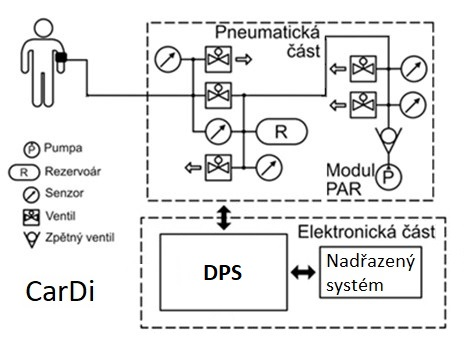
\includegraphics[width=1\textwidth]{pictures/blokove_schema_cele_zarizeni.jpg}
    \caption{Blokové schéma zařízení}
\end{figure}
Součástí pneumatické časti je uzavírací ventil, regulační ventily na obou částí uzavíracího ventilu, rezervoáru a klinicky validovaného modulu pro měření tlaku.
K elektrické části patří obvody pro ovládání regulačních a uzavíracího ventilu, komunikace s modulem pro měření tlaku, sběr dat ze senzorů tlaku na obou částí uzavíracího ventilu, komunikace a sběr dat z 24 bitového analogově digitálního převodníku a
uložení a čtení dat do přidané FLASH paměti.
\section{Řídící jednotka}

Řídící jednotka působí jako centrum řízení a sběru dat. Má na starosti řízení ventilů, natlakování pneumatického systémum, sběr a vyhodnocení
dat ze senzorů a komunikaci s nadřazeným systémem. \par

Jako řídící jednotka byl vybrán mikroprocesor STM32F407ZG (dále jenom MCU) od firmy ST Microelectronics.
Jádro je Arm® Cortex®-M4 32bit, jehož časovací frekvence může být až $168 \ MHz$. Jádro Cortex-M4 je vhodné pro zpracování signálu díky zabudovanému výpočetnímu modulu Floating Point Unit(FPU) určené na
počítání s desetinými čísly a také řadou instrukcí určené specificky na zpracování signálu.
\begin{figure}[H]
    \centering
    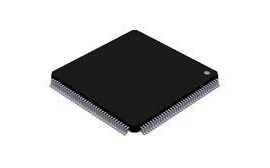
\includegraphics[width=0.5\linewidth]{pictures/stm32f407.jpg}
    \caption{Model STM32F407ZGT6 \cite{cite:STM32F407}}
    \label{fig:stm32}
\end{figure}
MCU je v obalu se 144 piny se 114 vstupně/výstupními piny, 1 MB FLASH paměti, 256 kB paměti SRAM, 3x 12 bit AD převodníky s až 24 kanály s maximální vzorkovací frekvencí 2.4 MHz,
2x 12 bit DA převodníky, 14 TIMER, 6x USART, 3x SPI, SysTick Timer, WatchDog a další periferie.
\par
Celkové zapojení MCU je na obrázku (\ref{fig:stm32_conection}).

\begin{figure}[H]
    \centering
    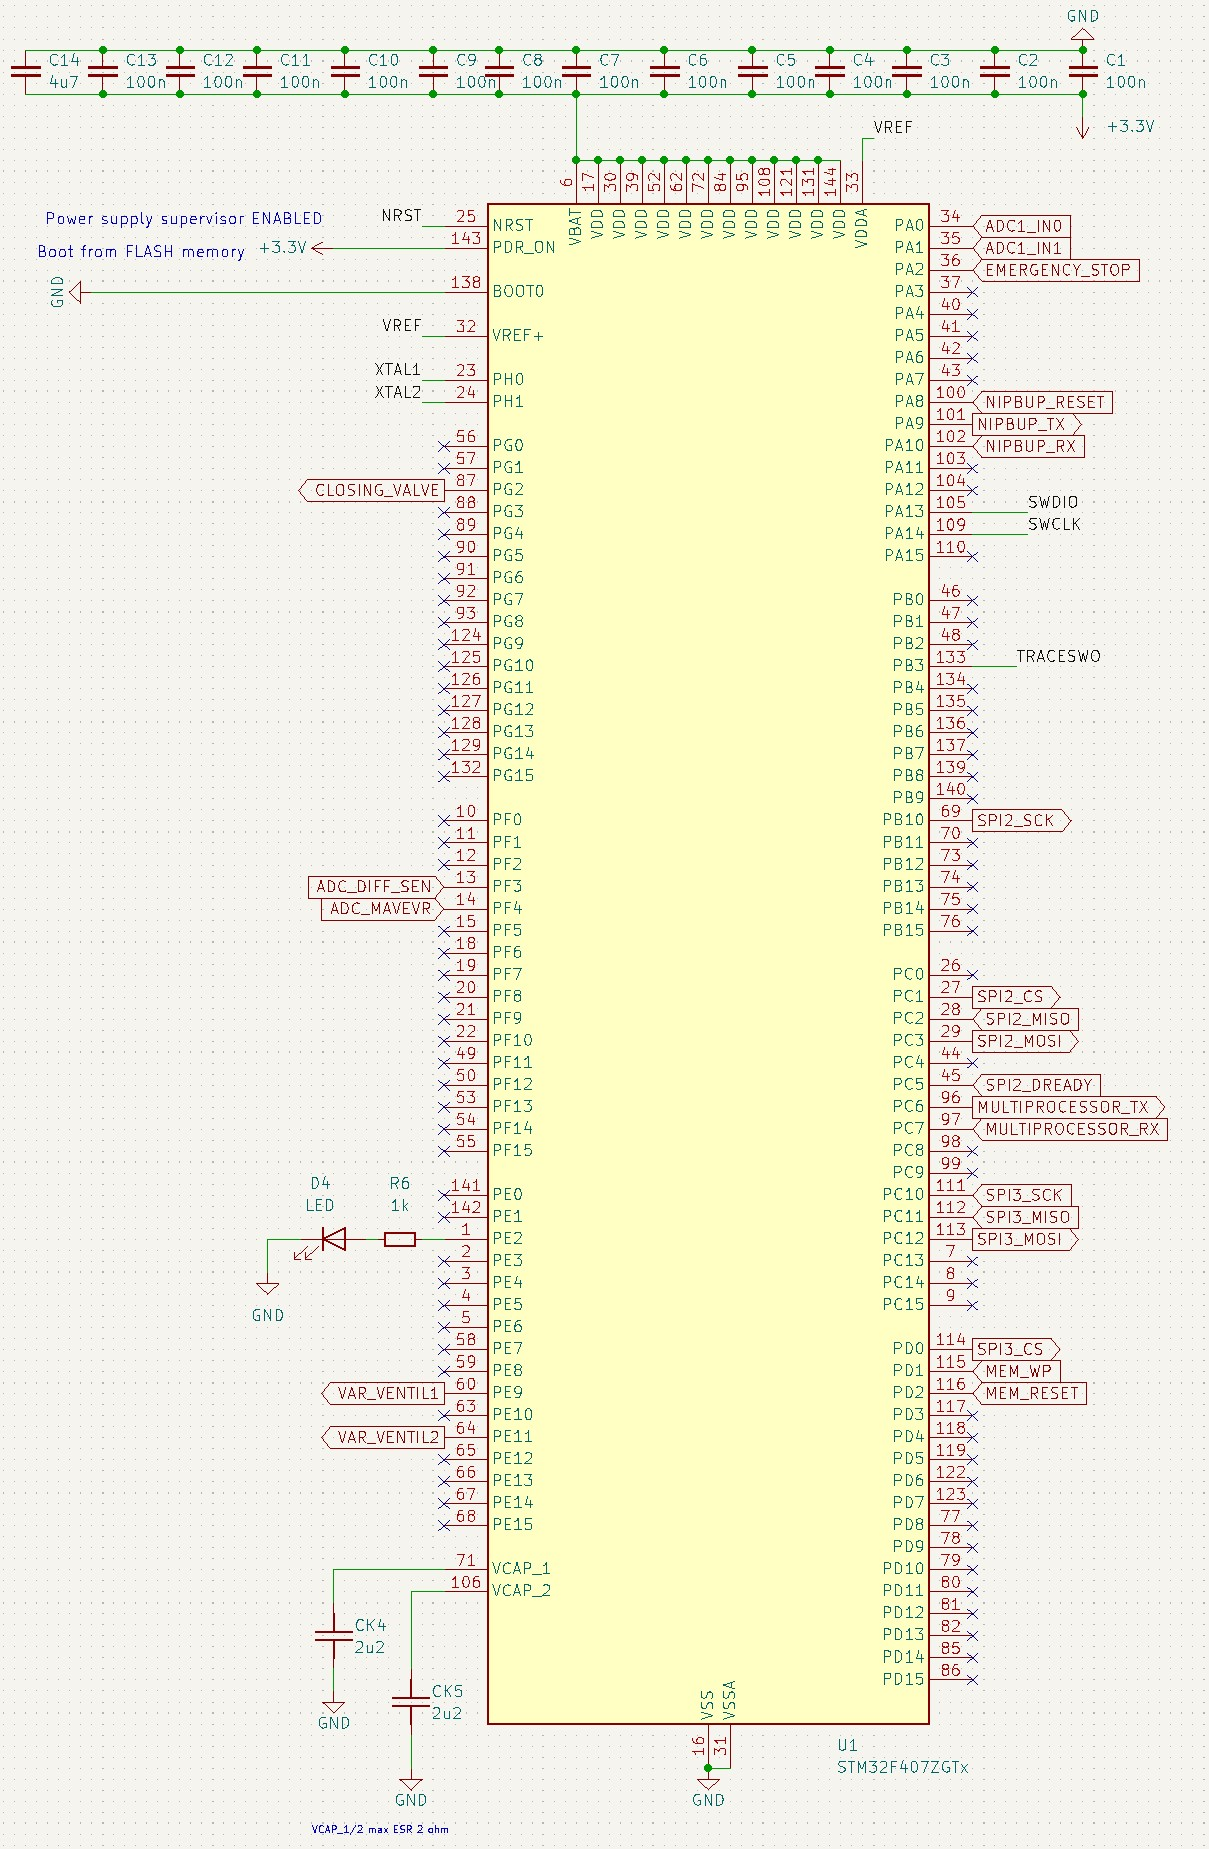
\includegraphics[width=1\linewidth]{pictures/stm_connection.jpg}
    \caption{Schéma zapojení STM32F407ZG}
    \label{fig:stm32_conection}
\end{figure}

Zapojení MCU je podle doporučeného zapojení. Jedná se hlavně o umístění a typy blokovacích kondenzátorů, reset signál, boot z interní nebo externí flash paměti a zvolení externích nízko a vysoko kmitočtových hodin. \par

\subsection{Externí hodiny}

MCU obsahuje interní vysokorychlostní RC oscilátor, ale pro maximální přesnost a spolehlivost byl zvolen externí vysokorychlotní oscilátor Abracon ABM3 o frekvenci  $8 \ MHz$. Externí oscilátor slouží jako hlavní časovací hodiny pro
jádro. Jádro může být na frekvenci až $168 \ MHz$ a to pomocí vnitřní násobičky frekvence Phase Locked Loop (dále pouze PLL) můžeme dosánout z $8 \ MHz$.

\begin{figure}[H]
    \centering
    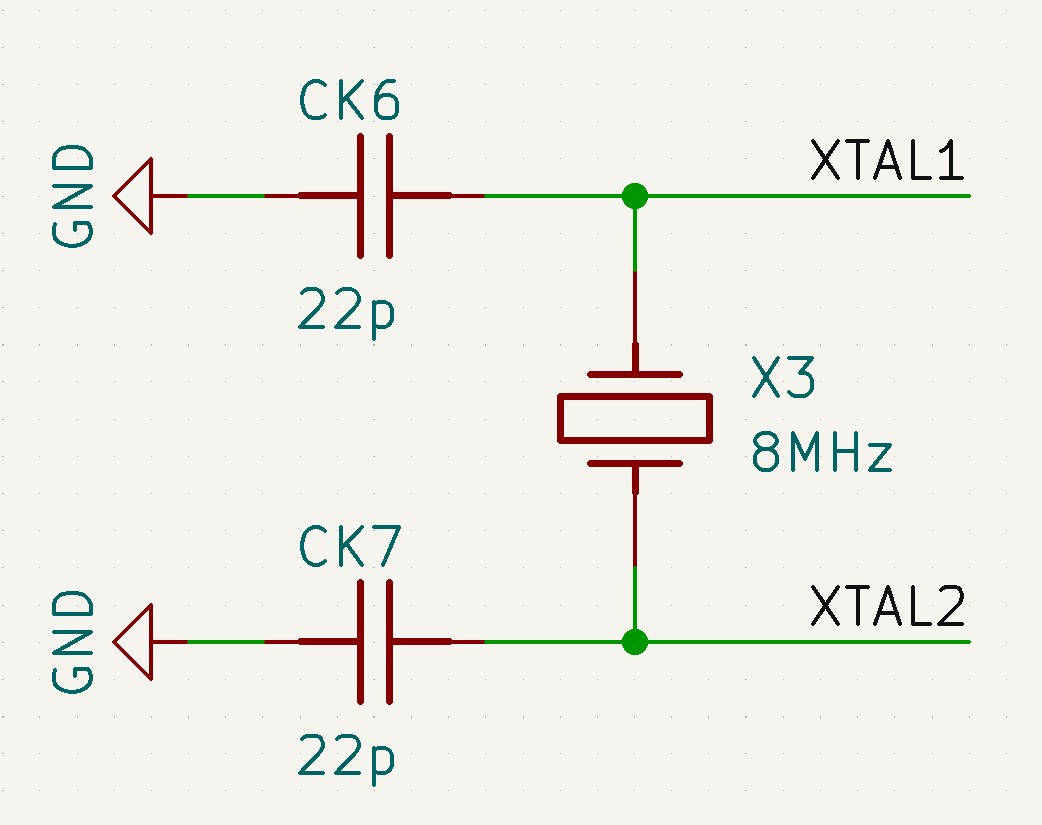
\includegraphics[width=0.8\linewidth]{pictures/stm32_hse.jpg}
    \caption{Schéma zapojení vysokorychlostního externího oscilátoru pro STM32}
    \label{fig:stm32_hse}
\end{figure}

Snížení frekvence externích hodin omezíme vysoko frekvečního rušení, případného přeslechu na vodičích a celkové signálové integritě.


\subsection{Napěťová reference pro analogové periferie} \label{section:vref}
Pro dosáhnutí nejpřesnějšího měření, je třeba, aby analogová čast byla co nejméně zarušena. Díky vysokým kmitočtům digitální čast MCU může zarušit analogové periférie a proto jsou v MCU digitální a analogové obvody oddělené.
Jako refereční napětí je použito zapojení na obrázku (\ref{fig:stm32_vref}).

\begin{figure}[H]
    \centering
    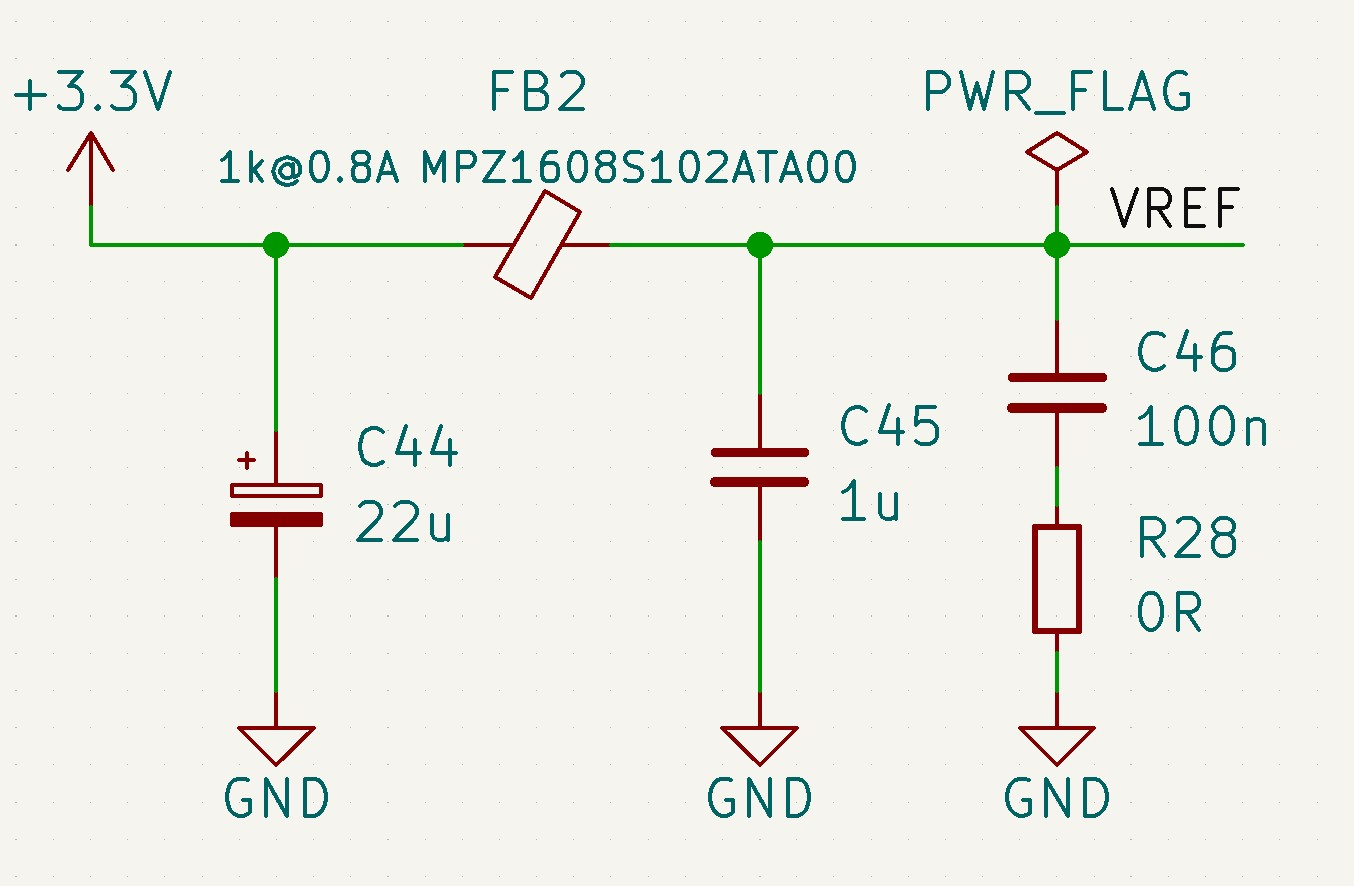
\includegraphics[width=0.9\linewidth]{pictures/stm_analog_reference.jpg}
    \caption{Schéma zapojení referečního napájení pro analogové periférie MCU}
    \label{fig:stm32_vref}
\end{figure}

Tento filtr začne potlačovat na frekvenci $f = 138 \ kHz$. Ale mezi $\approx 50 \ kHz$ a $ \approx 115 \ kHz$ filtr zesiluje, kde největší zesílení o $19 \ dB$ je na frekvenci $88.8 \ kHz$

\begin{figure}[H]
    \caption{Aproximace frekveční odezvy filtru pro refereční napájení analogové periférie MCU.}
    \label{fig:stm32_vref_response}
    \begin{tikzpicture}
        \begin{axis}[
                width=\linewidth,
                xmode = log,
                % ymode = log,
                % title = {Picture 1},  % whatever name you want
                ylabel = {(dB)},
                xlabel = {$f$ (Hz) },
                grid=both, % Display a grid
                grid style={dashed,gray!30}, % Set the style  
                % xunit = \si{s},
                % ymin = -3, ymax = 3,
                % minor y tick num = 1,
            ]
            \addplot[width=1pt,color=blue] table {graphs/vref_filtering_cardi.dat};
        \end{axis}
    \end{tikzpicture}
\end{figure}

% \begin{figure}[H]
%     \centering
%     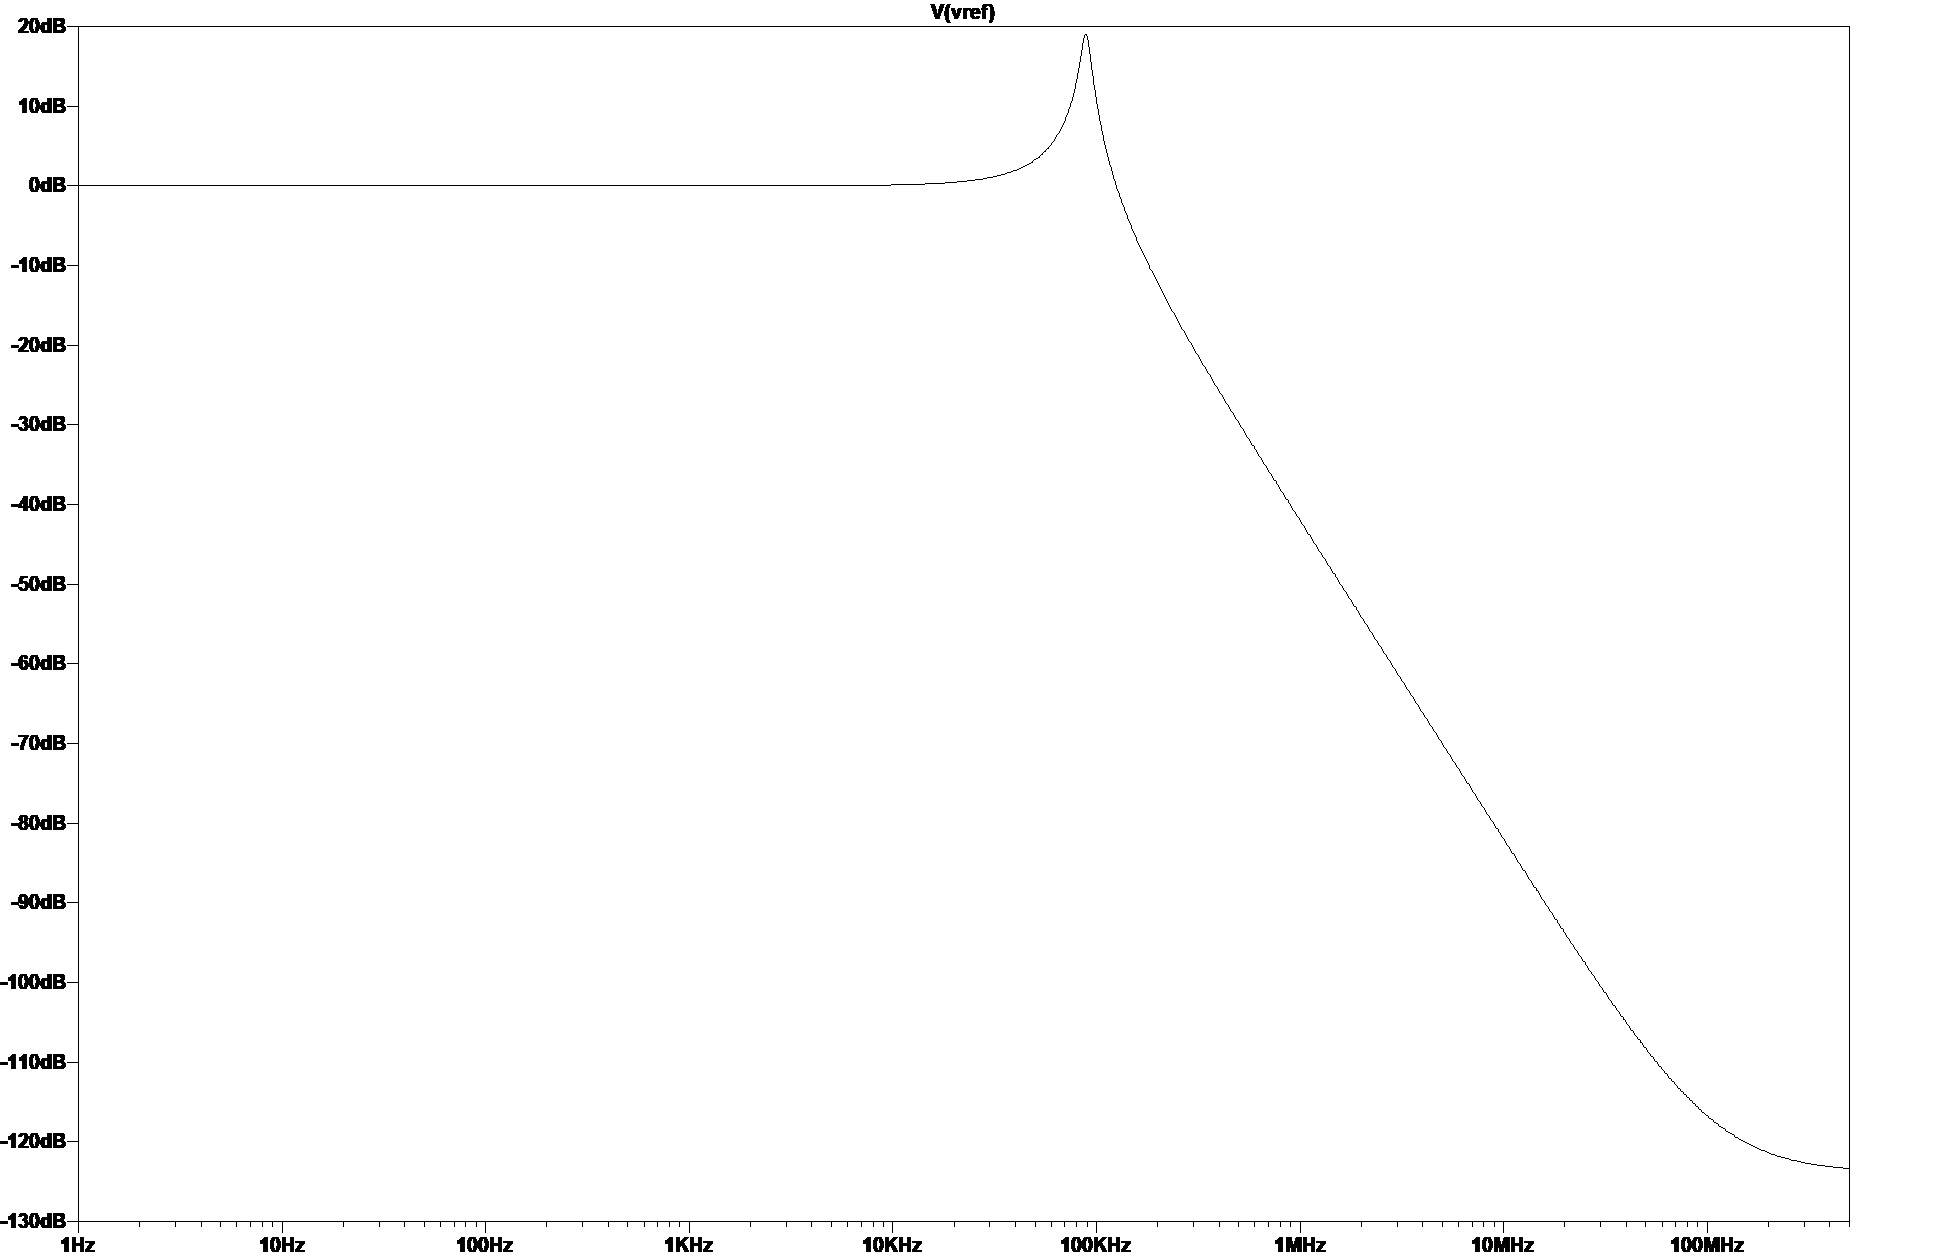
\includegraphics[width=1\linewidth]{pictures/cardi_vref_filter_response.jpg}
%     \caption{Aproximace frekveční odezvy filtru analogového napětí.}
%     \label{fig:stm32_vref_response}
% \end{figure}

Feritový korálek je pasivní součástka, který se používá pro filtraci vysokofrekvenčního rušení přes širokou část frekvenčního rozsahu. Největší impedanci má okolo určené frekvence a disipuje energii rušení ve formě tepla.
\subsection{Ochrana proti elektrostatickému výboji}
Elektrostatický výboj(ESD) je náhlý a krátkodobý elektrický proud mezi dvěma objeky s různým elektrickým potenciálem. Představuje horzbu elektrickým komponentům ve formě trvalého, nevratného poškození. Nejčastější místa probití jsou zejména místa, kterých se často dotýkáme například kontektory.
\par
Jako ochrana je použita transient voltage suppression (TVS) dioda D5V0F1U2S9-7 od firmy Diodes Incorporated.

\begin{figure}[H]
    \centering
    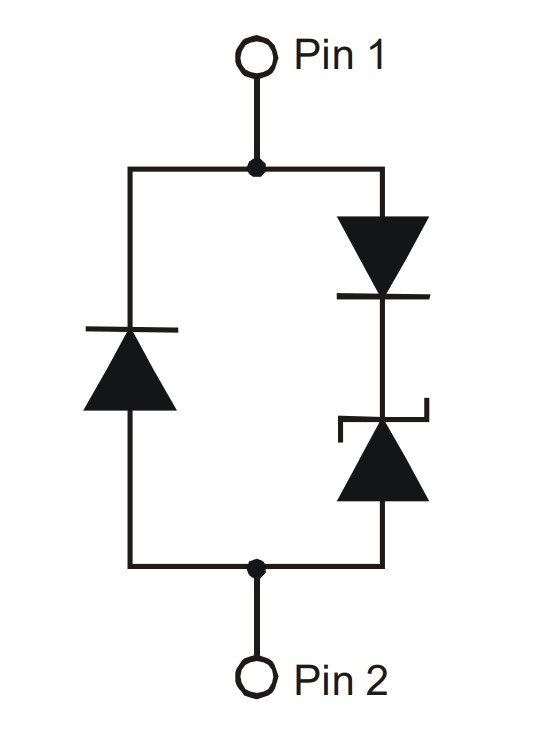
\includegraphics[width=0.4\linewidth]{pictures/esd_diode_schema.jpg}
    \caption{Schéma ochrané ESD diody D5V0F1U2S9-7. Kde Pin 1 je katoda. \cite{cite:ESD}}
    \label{fig:esd_diode}
\end{figure}

Tato dioda je určená pro ochranu proti elektrostatickým výbojům. Je připojena v závěrném směru na všechny konketory. V závěrném směru bude otevřena při napětí
$U = 5.5 \ V $ a napětí omezí na $U_{BR} = 6.0 \ V $.

\section{Modul měření krevního tlaku}

Součástí pneumatické části je modul PAR Medizintechnik NIBP 2020 UP , který omužňuje validované měření krevního tlaku oscilometrickou metodou v průběhu nafukování, také vyfukování, a následné nafouknutí na suprasystolický tlak. Samotné nafukování pneumatického systému je realizováno z elektromechanické vzduchové pumpy integrované v modulul PAR.
Pneumatická část modulu PAR se skládá ze vzduchové pumpy se zpětným ventilem zamezujícím úniku tlaku, vypouštějícího ventilu, tlakového senzoru a také redundantním sensorem tlaku a vypouštěcím ventilem pro případ poruchy. \par
Modul PAR má klinickou validaci pro měření krevního tlaku dle norem EN 80601-2-30, EN 81060-2 a systém podle norem EN 60601-1 (2. a 3. edice), EN 60601-1-2, EN 60601-1-6.
\begin{figure}[H]
    \centering
    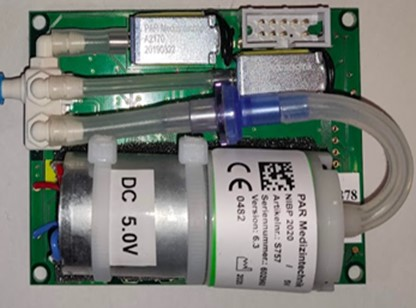
\includegraphics{pictures/par_nibp_up.jpg}
    \caption{Tlakový modul PAR NIBP 2020 UP}
    \label{fig:par_modul}
\end{figure}

Pneumatická část je řízena procesorem, se kterým lze komunikovat pomocí datové sériové linky RS232 či TTL a standardního protokolu CAS s rychlostí 4800 baud. Do modulu jsou posílány přes rozhraní UART příkazy pro nastavení režimu a parametrů zakončené příkazem pro zahájení měření.
\begin{figure}[H]
    \centering
    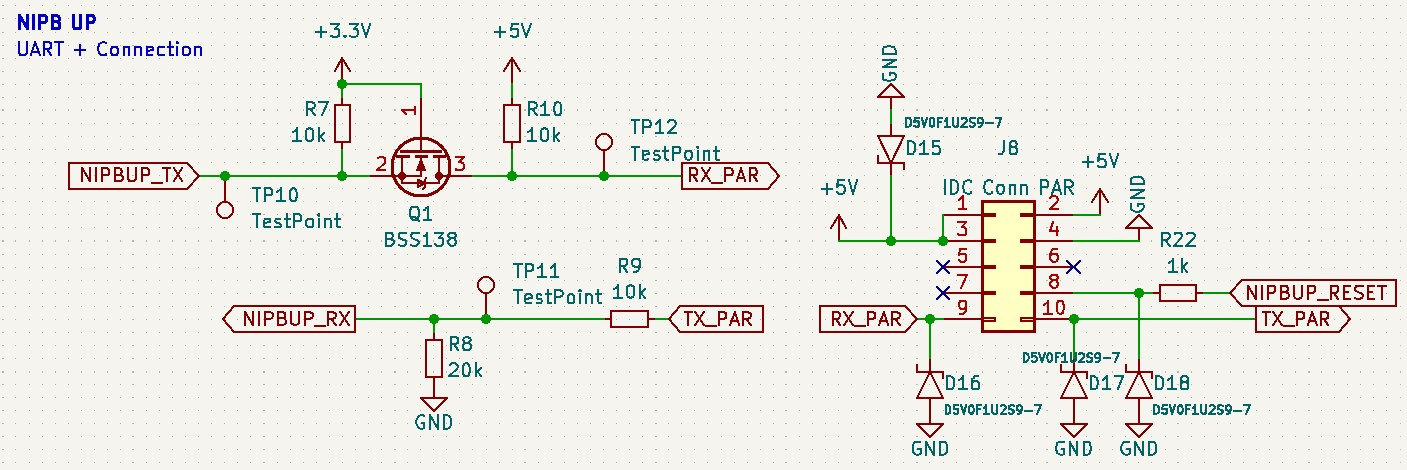
\includegraphics[width=0.9\linewidth]{pictures/nibpup_connection.jpg}
    \caption{Schéma připojení komunikační linky k MCU a napájení pro PAR NIBP 2020 UP }
    \label{fig:par_modul_comm}
\end{figure}
Pneumatickou část lze udržovat na hladinách tlaku v rozmezí (0–300) mmHg po dobu až 180 s a uživateli umožňuje zvolit odstup suprasystolického tlaku od naměřeného systolického tlaku. Po odeslání příkazu pro zahájení měření posílá modul po lince aktuální stav pneumatické části během celého měření a po měření posílá zprávu s naměřenými hodnotami krevního tlaku a srdeční frekvence.
\section{Senzory}
Tato sekce se zaměří na popis a použití senzorů a to zejména tlakových. Tlakové senzory tvoří nezbytnou část celkového přistroje a rozhodují o celkovém konfortu pacienta a také o přesnost výsledné terapie. \par
Parametry senzorů tlaku vychází z parametrů terapie. Pneumatický systém může být pod tlakem až $300 \ mmHg = 40 \ kPa$, tento požadavek musí splňovat všechny senzory napojené do pneumatického systému.

\subsection{Senzor tlaku} \label{section:pressure_sen}
Senzor tlaku se používá na snímání tlaku v jednotlivých větví pneumatického systému. \par

Použité sensory tlaku jsou NPX MP3V5050GC6U.

\begin{figure}[H]
    \centering
    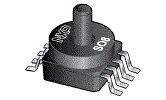
\includegraphics[width=0.5\linewidth]{pictures/nxp_sensor.jpg}
    \caption{Senzor tlaku NPX MP3V5050GC6U \cite{cite:NXP}}
    \label{fig:nxp}
\end{figure}

Je to analogový sensor tlaku od firmy NXP ze série peizorezistivních převodníků. Parametry jsou následovné:
\begin{table}[H]
    \label{tab:nxp_properties}
    \caption{Charakterisitky senzoru NPX MP3V5050GC6U. \cite{cite:NXP}}
    \begin{ctucolortab}
        \begin{tabular}{ccccccc}
            \toprule
            Charakteristika                                         & Symbol        & Min & Typ   & Max        & Jednotka         & \\ \midrule
            Rozsah tlaku                                            & $P$           & 0   & -     & 50         & $kPa$            & \\
            Vstupní napětí                                          & $U_{s}$       & 2.7 & 3.0   & 3.3        & $V$              & \\
            Vstupní proud                                           & $I_{s}$       & -   & 7     & 10         & $mA$             & \\
            Napěťový offset($0^{\circ}$ až $ 85^{\circ}  C $)       & $U_{off}$     & -   & 0.188 & -          & $V$              & \\
            $\textnormal{Full Scale Output}^{(\ref{enum:nxp_fso})}$ & $U_{FSO}$     &     & 2.77  &            & $V$              & \\
            Přesnost($0^{\circ}$ až $ 85^{\circ} C$)                & -             & -   & -     & $\pm 2.5 $ & $\%$             & \\
            Citlivost                                               & $\frac{U}{P}$ & -   & 54    & -          & $\frac{mV}{kPa}$ & \\
            \bottomrule
        \end{tabular}
    \end{ctucolortab}

    \begin{enumerate}
        \item \label{enum:nxp_fso} Maximální napětí při největším hodnoceném tlaku.
    \end{enumerate}
\end{table}

Zapojení senzoru je na separátní DPS podle doporučeného schématu (\ref{fig:nxp_recommended}) z katalogového listu.
\begin{figure}[H]
    \centering
    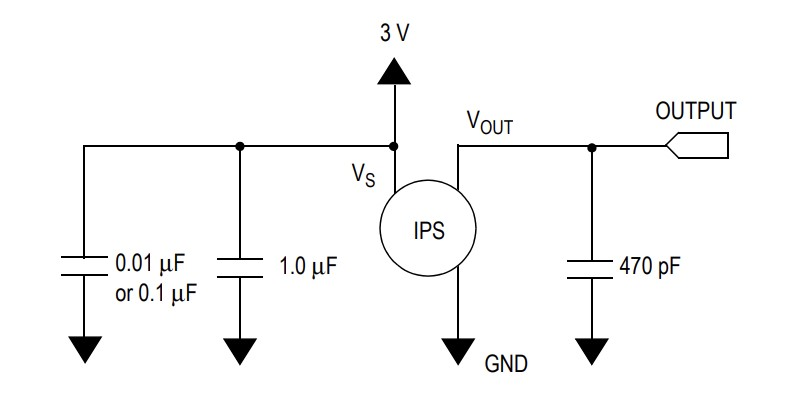
\includegraphics[width=0.9\linewidth]{pictures/nxp_recommended.jpg}
    \caption{Doporučené schéma zapojení senzoru tlaku NPX MP3V5050GC6U. Kde $V_S$ je vstupní napájecí napětí a $V_{out}$ je výstupní napětí.  \cite{cite:NXP}}
    \label{fig:nxp_recommended}
\end{figure}
Analogový výstup ze sensoru je připojen na interní AD převodník MCU.
\subsubsection{Převodní charakteristika}
Převodní charakteristika výstupního napětí $U_{o} \ V$ na tlak $P \ kPa$je
\begin{equation}
    P = \frac{U_o \pm ERROR}{0.018 \cdot U_s} - \frac{0.04}{0.018}
    \label{eq:nxp_transfer}
\end{equation}

\begin{figure}[H]
    \centering
    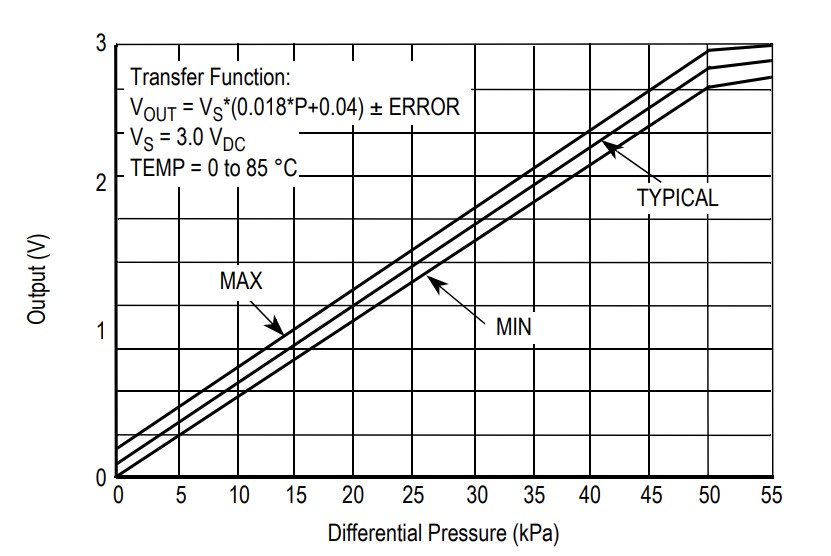
\includegraphics[width=0.9\linewidth]{pictures/nxp_transfer.jpg}
    \caption{Graf převodní rovnice tlak na napětí pro senzor tlaku NPX MP3V5050GC6U. \cite{cite:NXP}}
    \label{fig:nxp_transfer}
\end{figure}

\subsection{Diferenční sensor tlaku} \label{section:diff_pressure_sen}
Diferenční sensor tlaku slouží na snímání malých tlakových pulzací. Porovnává tlak mezí první a druhou (referenční) větví systému. Po natlakování pneumatického systému až na $300 \ mmHg$ uzavírací ventil oddělí systém na dvě větve. Rozdíl tlaků ve větvi může být $300 \ mmHg$ neboli $40 \ kPa$. \par
Diferenční sensor tlaku byl zvolen Amphenol ELVH-L02D-HRRD-C-NAA4. Je to analogový senzor tlaku určený na snímání ultra nízkých tlaků.
\begin{figure}[H]
    \centering
    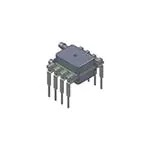
\includegraphics[width=0.4\linewidth]{pictures/amphenol.jpg}
    \caption{Diferenční sensor tlaku Amphenol ELVH-L02D-HRRD-C-NAA4 \cite{cite:Allsensors}}
    \label{fig:amphenol}
\end{figure}


\begin{table}[H]
    \label{tab:amphenol_properies}
    \caption{Charakterisitky diferenčního tlakového sensoru Amphenol ELVH-L02D-HRRD-C-NAA4 \cite{cite:Allsensors}}
    \centering
    \begin{ctucolortab}
        \begin{tabular}{ccccccc}
            \toprule
            Charakteristika                                                         & Symbol    & Min     & Typ        & Max         & Jednotka & \\ \midrule
            Rozsah tlaku                                                            & $P$       & -497.68 & -          & 497.68      & $Pa$     & \\
            $\textnormal{Proof pressure}^{(\ref{enum:amp_proof_pressure})}$         & $P_{pp}$  & -       & 67         & -           & $kPa$    & \\
            $\textnormal{Průrazný tlak}^{(\ref{enum:amp_burst_pressure}) }$         & $P_{bp}$  & -       & 103        & -           & $kPa$    & \\
            $\textnormal{Common mode pressure}^{(\ref{enum:amp_common_pressure})} $ & $P_{cm}$  & -       & 103        & -           & $kPa$    & \\
            Vstupní napětí                                                          & $U_{s}$   & 3.0     & 3.3        & 5.0         & $V$      & \\
            Vstupní proud                                                           & $I_{s}$   & -       & 2.1        & 2.8         & $mA$     & \\
            Napěťový offset                                                         & $U_{off}$ & -       & 1.65       & -           & $V$      & \\
            $\textnormal{Full Scale Span}^{(\ref{enum:amp_fss})} $                  & $U_{FSS}$ &         & $\pm 1.32$ &             & $V$      & \\
            Přesnost                                                                & -         & -       & -          & $\pm 0.25 $ & $\%$     & \\
            Citlivost                                                               & -         & -       & 0.2        & -           & $\%$     & \\
            \bottomrule
        \end{tabular}
    \end{ctucolortab}
    \begin{enumerate}
        \item \label{enum:amp_proof_pressure} Maximální tlak, který může být aplikován na jeden z portů senzoru a zachoval původní specifickace.
        \item \label{enum:amp_burst_pressure} Maximální tlak, který může být aplikován na jeden z portů senzoru, bez způsobení úniku tlaku.
        \item \label{enum:amp_common_pressure} Maximální tlak, který může být aplikován na oba porty zároveň, bez způsobení úniku tlaku.
        \item \label{enum:amp_fss} Algebraický rozdíl napětí při nejmenším možném specifikovaném tlaku a při maximálním specifikovaném tlaku.
    \end{enumerate}
\end{table}
\raggedbottom
Analogový signál ze senzoru je připojen k 24 bit AD převodníku přes RC článek. Schéma zapojení k AD převodníu je (\ref{fig:amphenol_circuit})

\begin{figure}[H]
    \centering
    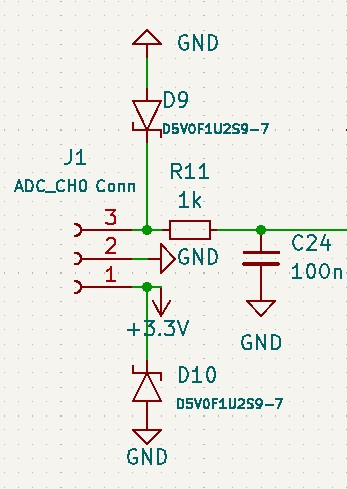
\includegraphics[width=0.7\linewidth]{pictures/diff_sen_circuit.jpg}
    \caption{Schéma zapojení diferenčního sensoru tlaku Amphenol ELVH-L02D-HRRD-C-NAA4 k AD převodníku.}
    \label{fig:amphenol_circuit}
\end{figure}

\raggedbottom
Zlomová frekvence RC článku $f_0 = \frac{1}{2 \pi RC} = 1591 \ Hz $ byla spočítána podle maximální frekvence tlakové vlny.

\begin{figure}[H]
    \centering
    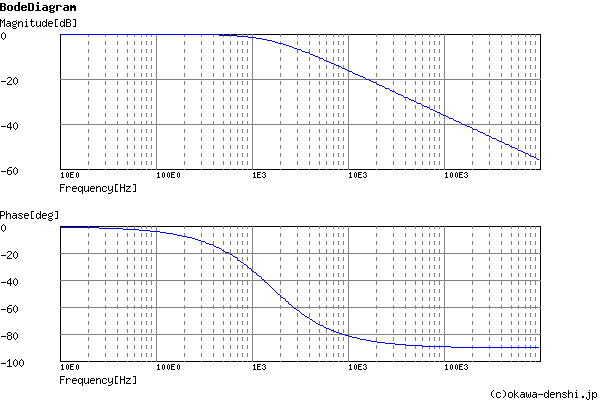
\includegraphics[width=0.9\linewidth]{pictures/rc_1k_100n_1591.png}
    \caption{Bodeho aproximace RC článku pro Amphenol ELVH-L02D-HRRD-C-NAA4. \cite{cite:RCResponse}}
    \label{fig:amphenol_filter}
\end{figure}

Podle Bodeho fázové aproximace RC článku na obrázku (\ref{fig:amphenol_filter}) můžeme vidět, že fáze se začne měnit před $\frac{f_0}{10}$.
Změna fáze snímaného signálu způsobí zkreslení výsledných hodnot a nepřesnou terapii.
\section{Vzduchové ventily}
Ventily jsou důležitou součástí pneumatického systému. Starají se o správný průběh terapie a také o bezpečí pacienta. \par
V systému rozlišujeme dva druhy vzduchových ventilů, uzavírací a vypouštějcí regulační. Uzavíraci ventil slouží pro oddělení manžety a pumpy. Vypouštěcí regulační ventily jsou na obou větvích pneumatického systému. Slouží jako pro regulaci tlaku v systému během terapie a také jako nouzové vypouštěcí ventily. \par
Všechny použité ventily nesmí v uzavřeném stavu propustit vzduch při tlaku $300 \ mmHg$, jinak by hrozilo nepřesné výsledky při měření a tím pádem špatná terapie.

\subsection{Uzavírací ventil}
Uzavírací ventil je důležitou součástí systému. Pneumatický systém rozdělí na dvě větve, kde jedna je část s manžetou a druhá větěv je jako referenční. \par

\begin{figure}[H]
    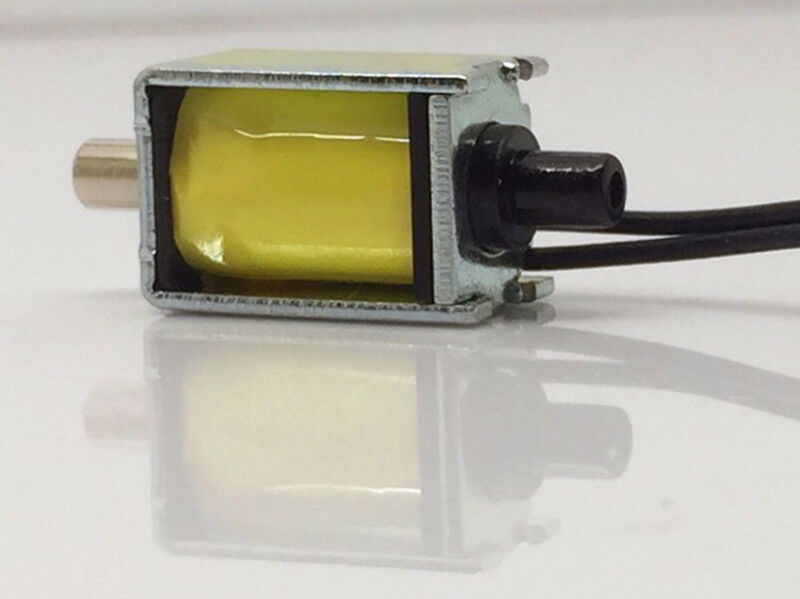
\includegraphics[width=0.9\linewidth]{pictures/closing_valve.jpg}
    \caption{Fotka uzavíracího ventilu CJAV08-2B05A1. \cite{cite:UzaviraciVentil}}
    \label{fig:closing_valve}
\end{figure}

Pro tento účel je použit ventil CONJOIN CJAV08-2B05A1. Je to řízený napětím, normálně zavřený, vzduchový ventil typu solenoid  o $U = 5 \ V$ a vstupní proud o $I = 204 \ mA \pm 10\% $ \cite{cite:UzaviraciVentil}

\begin{figure}[H]
    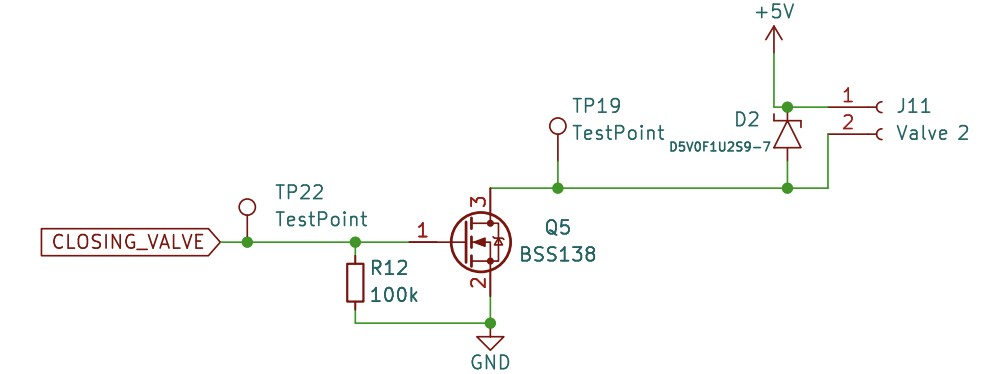
\includegraphics[width=0.9\linewidth]{pictures/closing_valve_driver.jpg}
    \caption{Schéma zapojení uzavíracího ventilu.}
    \label{fig:closing_valve_driver}
\end{figure}

Pro řízení ventilu z výstupního pinu MCU je použitý NMOS tranzistor BSS138. BSS138 má spínací práh napětí $U_{GS} = 3.3 \ V$ což je přímo výstupní napětí z GPIO a maximální proud přes drain je $I_D = 0.22 \ A$. Resistor přes Gate a Source zajisti známé napětí, pokud bude vstup na Gate plovoucí. Tím se zamezí neznámé chovaní tranzistoru.

\subsection{Regulační ventil}
Regulační ventily slouží k regulaci tlaku v systému při terapii a také jako vypouštěcí ventily pro vrácení pneumatického systému na atmosférický tlak. Ventily jsou umístěné na každe větvi pneumatického systému. Během terapie je možno si zvolit jak moc vysoký průtok vzduchu je možný, tím můžeme regulovat tlak v obou větvích podle potřeby terapie. \par

Regulační ventily jsou použité JQF4-6A/DC6V. Je to normálně otevřený lineární solenoid ventil. Maximální povolený tlak je $350mmHg$, řízený napětím $U = 6 \ V$ DC a proudový odběr je $I = 0.107 \ A$.\par

Napětí na ventilech je $5V$ i přes to, že ventily požadují napětí $6 \ V$. Sadou testů zjístilo, že momentální napětí vyhovuje naším požadavkům a únik tlaku při plném sevření nijak neovlivňuje terapii a přidáním $6 \ V$ by se akorát zvýšila komplexita systému.

\begin{figure}[H]
    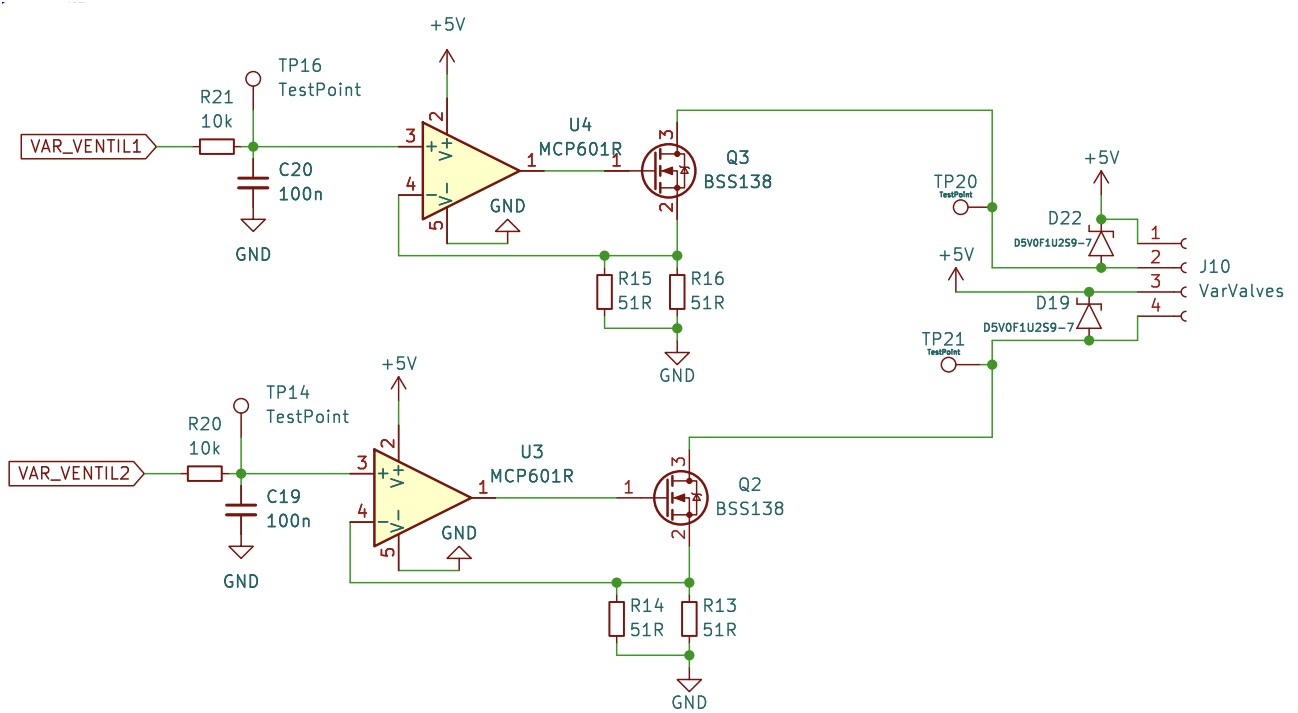
\includegraphics[width=1\linewidth]{pictures/var_valves.jpg}
    \caption{Schéma zapojení regulačních ventilů.}
    \label{fig:variable_valve_driver}
\end{figure}

\subsubsection{Zdroj proudu}
Regulační ventily jsou řízené napěťově řízeným zdrojem proudu jak je na obrázku (\ref{fig:variable_valve_driver}).\par
Ventily jsou napojené na drain NMOS tranzistoru, přes který jde konstatní napětí požadované ventilem. Proud se řídí operačním zesilovačem, který má na neinvertujícím vstupu $U_+$ napojené řídící napětí $U_i$. Výstup operačního zesilovače je spojen s gate tranzistoru. Source tranzistoru je spojen s invertujícím vstupem $U_-$ operačního zesilovače a také paralelně k zemi jsou zapojené resistory $R_{||}$, které určují maximální možný proud na regulačních ventilech. Výsledný proud je:
\begin{equation}
    \label{eq:current_source}
    I = \frac{U_i}{R_{||}}
\end{equation}
V případě na obrázku (\ref{fig:variable_valve_driver}) paralelní resistory $R_1 = R_2 = 51 \ \Omega$ mají výslednou hodnotu:
\begin{align*}
    R_{||} = \frac{R_1 R_2}{R_1 + R_2} = \frac{51}{2} = 25.5 \ \Omega
\end{align*}
Maximálním napětí, které umožní MCU z GPIO pinu je $3.3V$ proto maximální možný proud na regulačních ventilech je:
\begin{align*}
    I = \frac{U_i}{R_{||}} = \frac{3.3}{25.5} \approx 129 \ mA
\end{align*}

Pokud budeme brát v úvahu ideální OZ, tak do invertujícího $U_-$ a neinvertujícího $U_+$ vstupu jde nulový proud, kde $U_+ = U_-$ a výstup z OZ je
\begin{align}
    U_o = A(U_+ - U_-)
\end{align}
kde $A [-] $ je zesilovační činitel, který se blíží k nekonečnu. Pokud bude na výstupu OZ nulové napětí, tranzistor je uzavřen a napětí na source je také nulové. Pokud ale například dáme řídící napětí třeba na $U_i = 1V$, poté se OZ bude snažit, aby rozdíl $U_+ - U_- = 0$, tak na výstupu OZ se bude zvyšovat napětí dokud napětí na source nebude $U_- = U_i$. To znamená, že přes regulační ventily právě bude procházet proud z rovnice (\ref{eq:current_source}).

Použitý NMOS tranzistor je BSS138, který má minimální práhové napětí $U_{GS(th)} = 0.5 \ V$, to je napětí, při kterém začne protékat proud. To znamená, že minimální řídící napětí musí být $U_{i} = 0.5 \ V$


\subsubsection{Řídící signál}
Řídící signál je čtvercový pro řízení proudového zdroje. PWM signál z MCU o frekvenci $f_{PWM} = 25 kHz$ je filtrován pomocí RC článku o zlomové frekvenci $f_c = 159 Hz$, který slouží pro modulaci řídícího PWM signálu na konstatní napětí.
\par
Pulse Width Modulated(PWM) signál je periodický čtvercový signál s fixní periodou a měnící se poměrem času v log.1 a log.0, také nazývané jako střída(Duty Cycle). Průměrné napětí PWM signálu je
\begin{equation}
    U_{out} = U_{max} \cdot Duty Cycle
\end{equation}
kde $U_{max}$ je maximální amplituda PWM signálu. \par


Pomocí fourierovy analýzy PWM signálu můžeme vidět, že PWM signál se neskládá pouze z jedné frekvence, ale z mnoha (\ref{fig:pwm_spectrum}).

\begin{figure}[H]
    \centering
    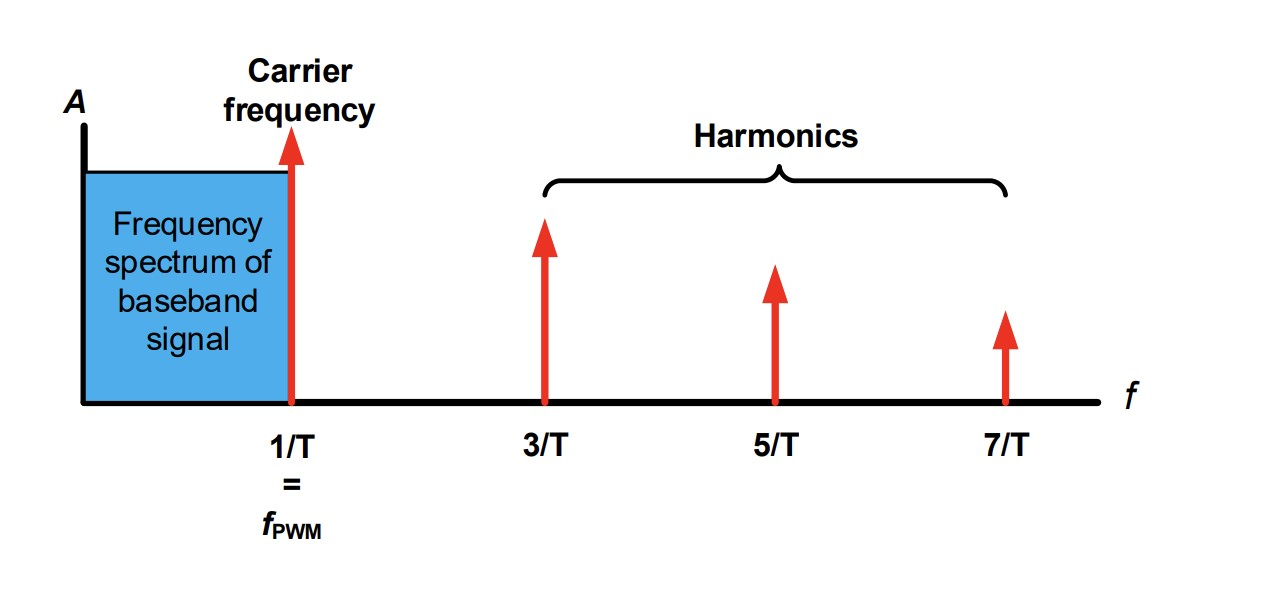
\includegraphics[width=1\linewidth]{pictures/pwm_spectrum_microchip90003250A.jpg}
    \caption{Spektrum PWM signálu převzatého od Microchip TB3250 kde $f_{PWM}$ je frekvence PWM signálu a $T$ je jeho perioda. \cite{cite:MCPPWV}}
    \label{fig:pwm_spectrum}
\end{figure}

Největší amplitudu typyckého PWM signálu má na její nastavené frekvenci $f_{PWM}$ a ostatní harmonické frekvence jsou její celočíselné násobky. Tyto frekvence přidávají nechtěný šum a můžou být potlačeny pomocí filtru typu dolní propust.


\begin{figure}[H]
    \centering
    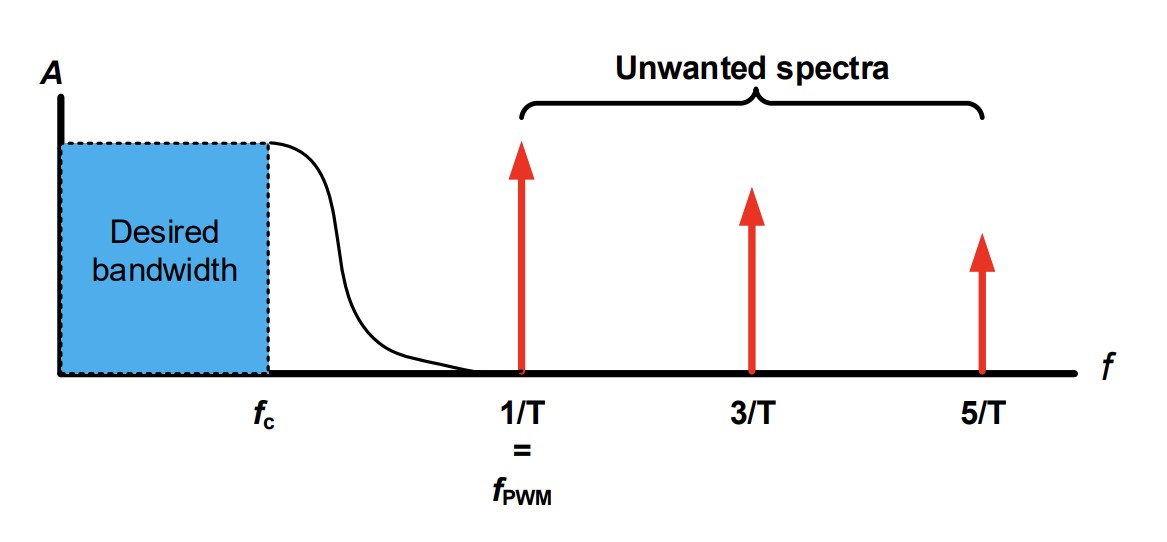
\includegraphics[width=1\linewidth]{pictures/rc_pwm_spectrum_microchip90003250A.jpg}
    \caption{Požadované odstraněné frekvence ve spektru PWM signálu převzatého od Microchip TB3250 kde $f_{PWM}$ je frekvence PWM signálu a $T$ je jeho perioda, $f_{c}$ je zlomová frekvence filtru.\cite{cite:MCPPWV}}
    \label{fig:unwanted_pwm_spectrum}
\end{figure}

Použitá dolní propust je RC filtr. Podle obrázku (\ref{fig:variable_valve_driver}) RC filtr je složený z odporu $R = 10 \ k\Omega$ a kondenzátoru $C = 100 \ nF$ kde výstupní napětí je napětí na kondenzátoru.
Kde $f_c = 159 \ Hz$ je zlomová frekvence filtru.

\begin{figure}[H]
    \centering
    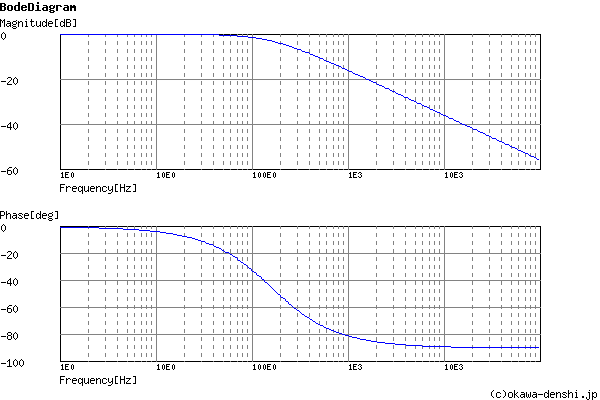
\includegraphics[width=1\linewidth]{pictures/var_rc_filter.png}
    \caption{Frekveční charakteristika použitého RC filtru pro převod PWV na napětí.\cite{cite:RCResponse}}
    \label{fig:var_rc_filter_char}
\end{figure}

Na obrázku (\ref{fig:var_rc_filter_char}) můžeme vidět, že signál se začne atenuovat na zlomové frekvenci a fáze signálu se začne posouvat na frekvenci $\frac{f_c}{10}$.  \par

Aby výstupní řídící signál byl co nejvíce konstatní musíme zvolit vstupní frekvenci PWM signálu co nejvyšší, aby harmonické složky byly co nejvíce utlumeny.

\begin{figure}[H]
    \caption{Simulace RC filtru při vstupním PWM signálu o střídě $50\%$ a frekvencí $f_{PWM} = 168 \ kHz $. Simulace byla provedena v programu LTspice XVII.}
    \label{fig:filtered_pwm}
    \begin{tikzpicture}[spy using overlaysshadow={
                    magnification=3,
                    size=1.5cm,
                    connect spies}
        ]
        \begin{axis}[
            width=\linewidth,
            % title = {Picture 1},  % whatever name you want
            ylabel = {$U_{out}$ [V]},
            xlabel = {Čas [s]},
            grid=major, % Display a grid
            grid style={dashed,gray!30}, % Set the style  
            % xunit = \si{s},
            % ymin = -3, ymax = 3,
            % minor y tick num = 1,
            ]
            \addplot[blue] table {graphs/pwm_to_analog.dat};
            % \begin{scope}
            % \spy [red] on (6,8.5cm) in node at (6.5cm,7.25cm);
            % \spy [blue,size=1cm] on (3cm,1cm) in node  at (0,-1.25cm);
            % \end{scope}
        \end{axis}

    \end{tikzpicture}
\end{figure}

% \begin{figure}[H]
%     \centering
%     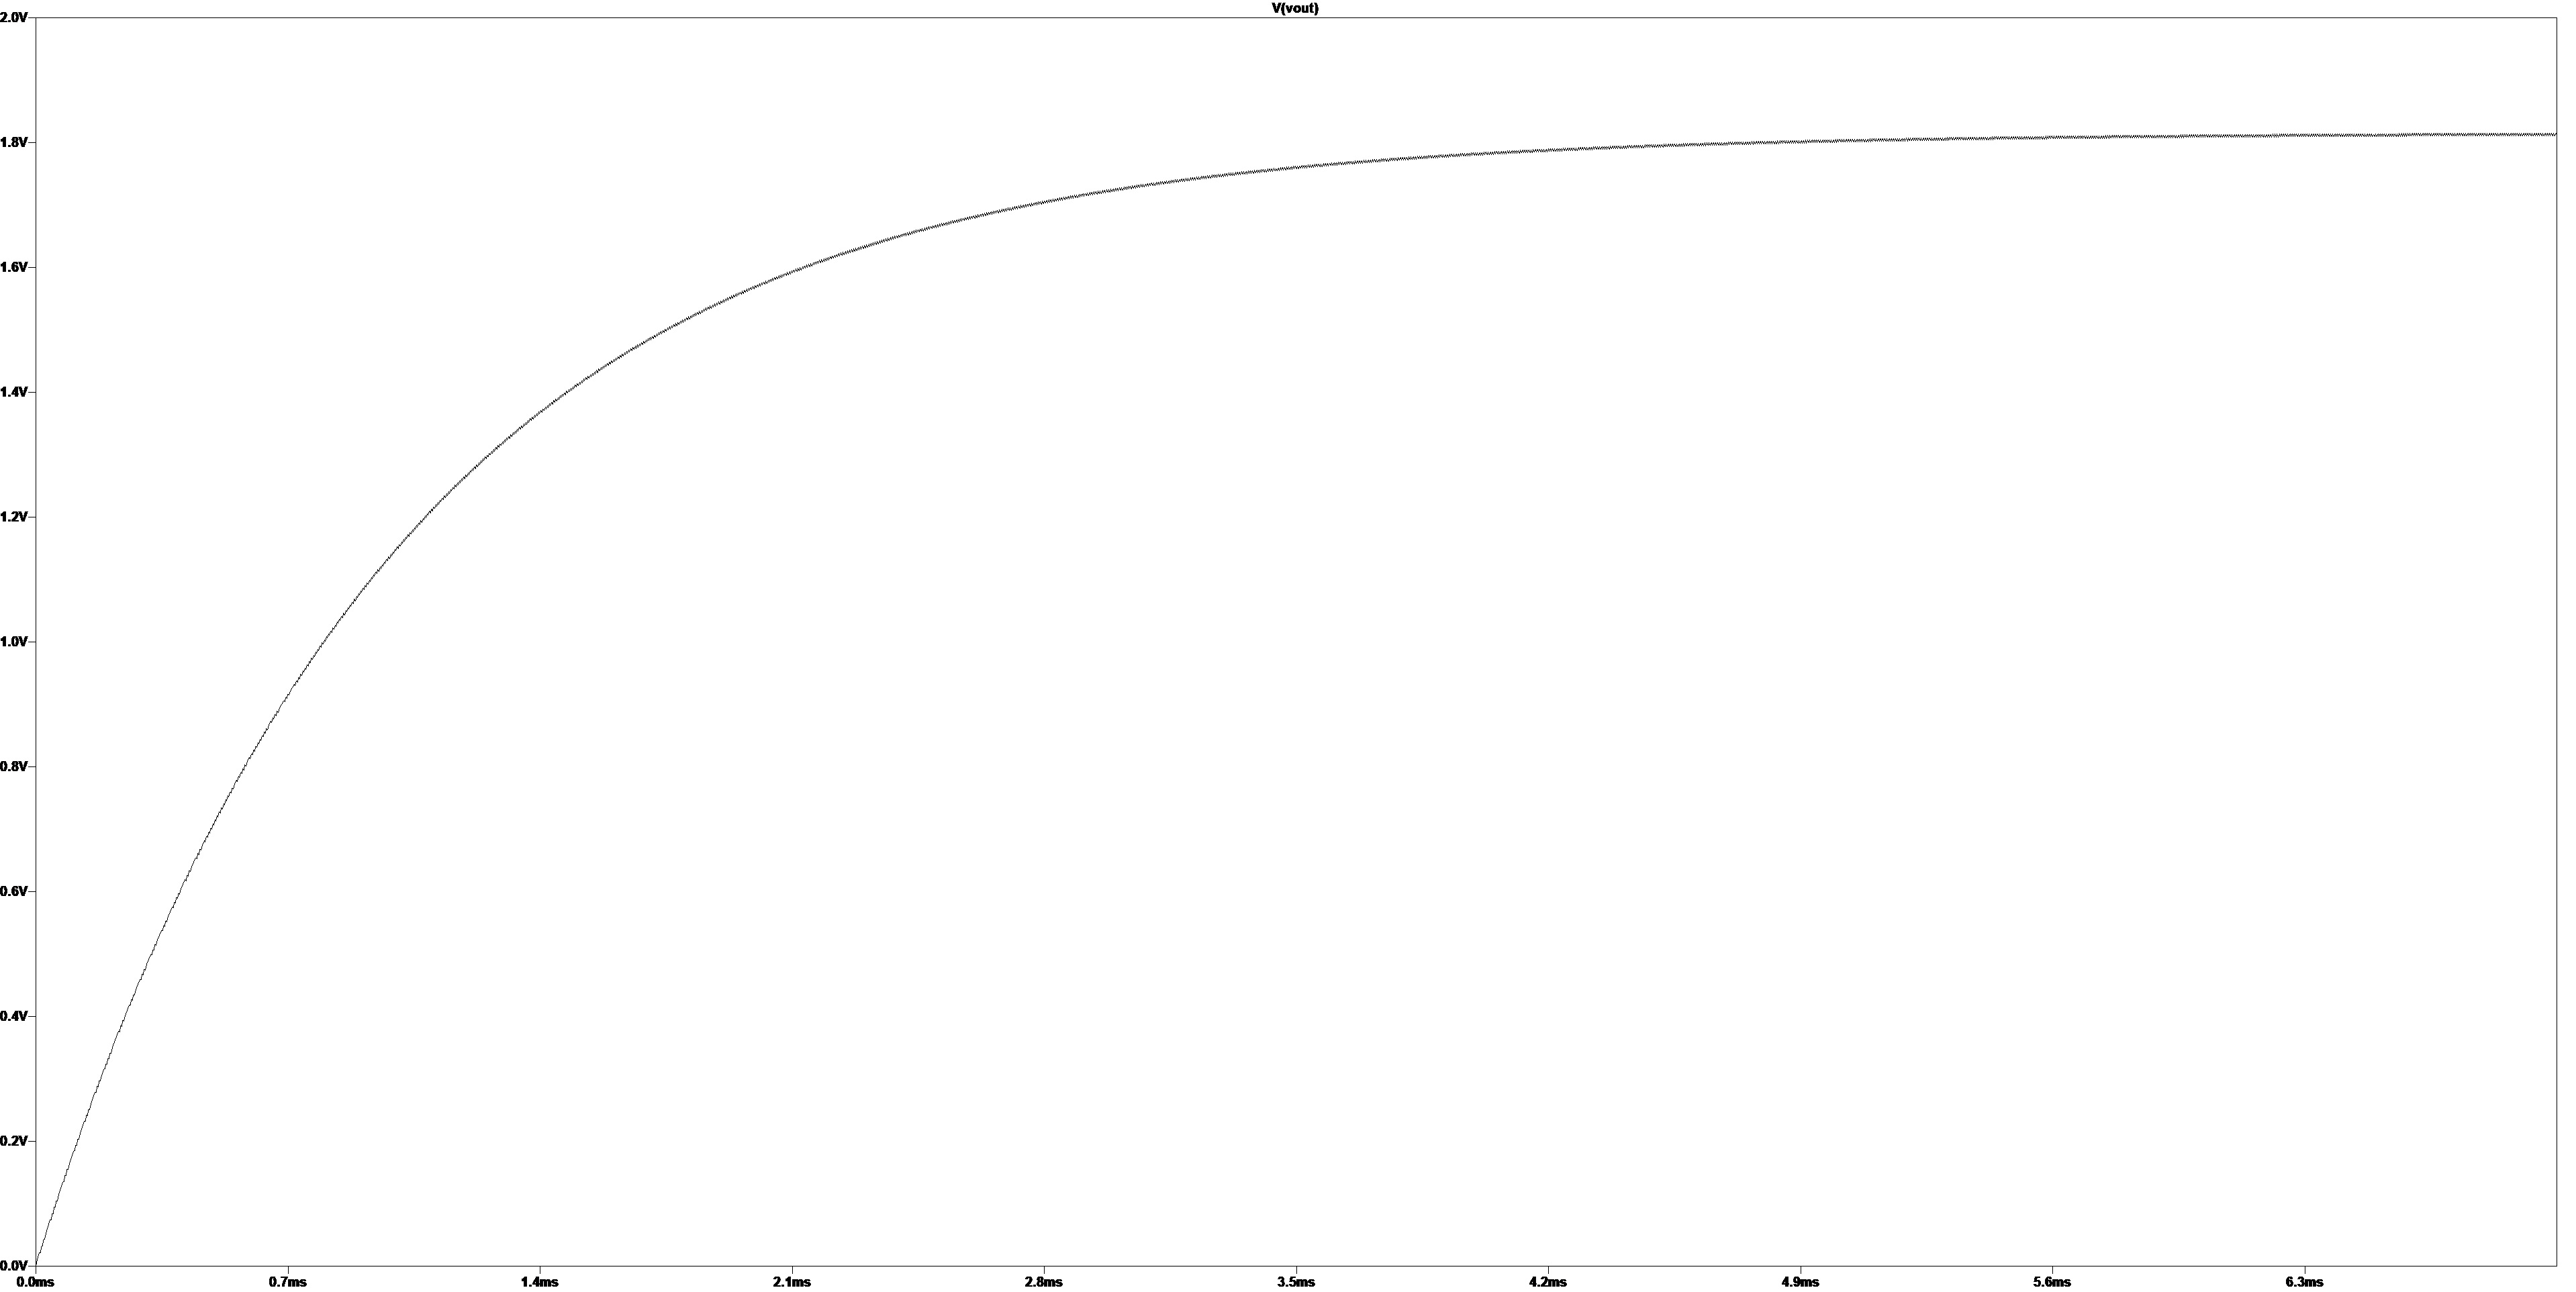
\includegraphics[width=1\linewidth]{pictures/filtered_pwm.jpg}
%     \caption{Simulace RC filtru při vstupním PWM signálu o střídě $50\%$ a frekvencí $f_{PWM} = 168 \ kHz $. Simulace byla provedena v programu LTspice XVII.}
%     \label{fig:filtered_pwm}
% \end{figure}

Rušení výstupního signálu ovlivní chování regulačního ventilu. Toto rušení způsobí periodickou změnu amplitudy výstupního signálu a regulační ventil se podle této amplitudy bude periodicky otevírat a zavírat. Při zvolené frekvenci PWM $f_{PWM} = 168000 \ Hz $ je změna napětí $\approx 2 \ mV$. To způsobý změnu proudu $I = \frac{0.030}{25.5} = 11 \ mA $. \par
Volba velikosti prvků RC článku ovlivní schopnost reakce na změnu vstupního napětí.
Časová konstanta $\tau = RC = 10 \times 10^{3} \cdot 100 \times 10^{-9}= 1\ ms$ definuje čas, který potrvá aby napětí na kondenzátoru dosáhlo $U_{C}(\tau) = U_{in}(\tau)(1 - e^{-1})$, což je $\approx 63 \ \% $ vstupního napětí $U_{in}$.

\par
Díky rovnici
\begin{equation} \label{eq:pwm_accuracy}
    2^N = \frac{f_{TIMCLK}}{f_{PWM}}
\end{equation}
můžeme získat přesnost střídy PWM signálu. $f_{TIMCLK} = 168 \ MHz$ je obnovovací frekvence periferie TIMER, který generuje PWM signál. Pokud rovnici (\ref{eq:pwm_accuracy}) vyřešme pro $N$ získáme rovnici pro počet bitů a přesnosti střídy PWM signálu.
\begin{equation}
    N = \frac{\log_{2} (\frac{f_{TIMCLK}}{f_{PWM}})}{\log_{2}(2)} = \frac{ARR}{\log_{2}(2)}
\end{equation}
$ARR$ je Auto-Reload-Register MCU pro daný TIMER. Podle nastavené hodnoty v $ARR$ je možné nastavit frekvenci PWM signálu. Pro tento připad $N \doteq 9.96 $ bit.

\section{Digitalizace analogových signálů}
Tato sekce popisuje typy použitých analogově digitálních převodníků, které jsou použity pro snímání analogových výstupů ze senzorů tlaku. Jsou použity dva typy AD převodníků, první je 12 bit AD převodník součástí MCU STM32F407ZG6 pro snímání napětí tlakových sezorů na větvích pneumatického systému popsaných v sekci (\ref{section:pressure_sen}).
Další je 24 bit sigma-delta AD převodník Microchip MCP3561 pro snímání napětí z diferenčního tlakového sensoru popsaný v sekci (\ref{section:diff_pressure_sen}).

\subsection{Snímání signálů z tlakových senzorů větví pneumatíckého systému}
Je použit AD převodník součástí periférii rodiny MCU STM32F4xx. Jedná se o 12 bitový AD převodník s postunout aproximací a maximální vzorkovací frekvencí $f_{sample} = 2.4 \ MSPS$. Pro každý kanál se může aplikovat jiná vzorkovací frekvence. \par
Díky měření pouze absolutní hodnoty tlaku ze senzorů vzorkovací frekvence nemusí být vysoká. Vzorkovací frekvence je:
\begin{equation}
    f_{sample}=\frac{f_{ADCCKL}}{vzorkovací \, čas + 15 \, cyklů } = \frac{20.5 \! MHz}{480 + 15} \approx 41.5 \; kHz
\end{equation}
Vzorkovací frekvence závisí na vstupní frekvenci AD převodníku $f_{ADCCKL} = 20.5 \ MHz$, minimální počet $f_{ADCCKL} $ cyklů pro převod je $15$ a vzorkovacím časem, které jsou předem dané výrobcem. Minimální vzorkovací čas je $3$ a maximální je $480$.
\par
Přesnost AD převodníku je $1 LSB = \frac{U_{ref}}{2^N} = \frac{3.3}{2^{12}} = 0.000805 \ \frac{V}{ADC \ krok}$ závisí na referečním napětí diskutovaném v sekci (\ref{section:vref}).

\begin{equation} \label{eq:max_adc_R}
    R_{AIN} = \frac{k - 0.5}{f_{ADCCLK} \cdot C_{ADC} \cdot ln(2^{N+2})} - R_{ADC}
\end{equation}
Rovnice (\ref{eq:max_adc_R}) slouží pro určení maximální vstupní externí impedance pro chybu pod $\frac{1}{4} \ LSB$. $N = 12$ je rozlišení AD převodníku, $k = 480$ je vzorkovací čas, $R_{ADC} = 6 \ k\Omega$ je vnitřní impedance vstupního kanálu AD převodníku a
$C_{ADC} = 4 \ pF$ je interní kapacita obvodu Sample and Hold. Výsledná maximální vstupní impedance je $R_{AIN} = 1.75 \ M\Omega$, ale podle katalogového listu je maximální externí impedance AD převodníku $R_{AIN} = 50 \ k\Omega$.
\par
K dalším chybám AD převodníku patří

\begin{table}[H]
    \label{tab:stm_adc_error}
    \caption{Charakteristika vestavěného AD převodníku v STM32F407ZG6}
    \hspace*{-1.3cm}
    \begin{ctucolortab}
        \begin{tabular}{ccccccc}
            \toprule
            Charakteristika               & Symbol & Testovací podmínky       & Typ       & $\textnormal{Max}$ & Jednotka & \\ \midrule
            Celková neupravená chyba      & $ET$   &                          & $\pm$ 2   & $\pm$ 5            &          & \\
            Napěťová nesymetrie           & $EO$   & $f_{ADC} = 30 \ MHz$     & $\pm$ 1.5 & $\pm$ 2.5          &          & \\
            Napěťový zisk                 & $EG$   & $R_{AIN} < 10 \ k\Omega$ & $\pm$ 1.5 & $\pm$ 3            & LSB      & \\
            Difereciální  chyba linearity & $ED$   &                          & $\pm$ 1   & $\pm$ 2            &          & \\
            Integrální chyba linearity    & $EL$   &                          & $\pm$ 1.5 & $\pm$ 3            &          & \\
            \bottomrule
        \end{tabular}
    \end{ctucolortab}
\end{table}

\subsection{Snímání signálů z diferenčního tlakového sensoru pneumatíckého systému} \label{section:mcp3561_hw}
Difereční sensor tlaku snímá dynamické jevy tlaku krevního řečiště. Při srdečním tepu např. 120 tepů/min tj. 2 Hz, odpovídá 20. harmonická složka signálu frekvenci  $f = 40 \ Hz$. Aby byl tlakový analogový signál správně převeden do digitálního signálu, musí být dodržen Nyquistův teorém.
\begin{equation} \label{eq:nyquist}
    f_s \geq 2f
\end{equation}
Rovnice (\ref{eq:nyquist}) říká, že vzorkovací frekvence musí být alespoň dvojnásobek snímaného signálu.
\par
Pro zachycení pulzní tlakové vlny je také zapotřebí dostatečné rozlišení v časové oblasti. Pokud vzorkovací frekvence signálu je $f_s = 5000 \ Hz$, chyba v měření může být $t_e = \pm 200 \ \mu s$. Podle vzroce (\ref{eq:pwv}) můžeme vypočítat chybu měření v závislosti na časovém kroku.
Například ať $l = 0.5 \ m$, $t_2 = 200 \ ms$ a $t_1 = 0 \ ms$, tak výsledné $PWV$ bude $PWV = 5 \ \frac{m}{s}$. Pokud započítáme chybu $t_e$ do vý počtu rychlost pulzní vlny bude
\begin{equation*}
    PWV = \frac{2l}{t_2 - t_1 + t_e} = \frac{1}{0.2 - 0.0002} = 5.005 \ \frac{m}{s}
\end{equation*}
\begin{equation*}
    PWV = \frac{2l}{t_2 - t_1 + t_e} = \frac{1}{0.2 + 0.0002} = 4,995 \ \frac{m}{s}
\end{equation*}
Výsledek se může lišit o $\pm 0.1 \ \%$.
\par
Byl vybrán 24 bit sigma-delta AD převodník MCP3561 od firmy Microchip s maximální vzorkovací frekvencí $153.6 \ kHz$. Je to AD převodník s velmi nízkým šumem, s jedním diferečním vstupem nebo dvěmi jednotlivými vstupy analogových signálu.
Obsahuje interní oscilátor, teplotní sensor, obvody pro detekci zkratu či odpojeného sensoru, programovatelné zesílení od $0.33 \times$ až $64 \times$ a další.
\par
MCP3561 komunikuje s MCU pomocí komunikačního rozhraní Serial Peripheral Interface (SPI) až s maximální rychlostí $20 \ MHz$. Komunikace probíha po 8 bitových slovech, kde odpovědi z AD převodníku můžou mít délku 8,24 a nebo podle kofigurace i 32 bit.
\begin{figure}[H]
    \centering
    \caption{Zapojení AD převodníku MCP3561}
    \label{fig:mcp3561_connection}
    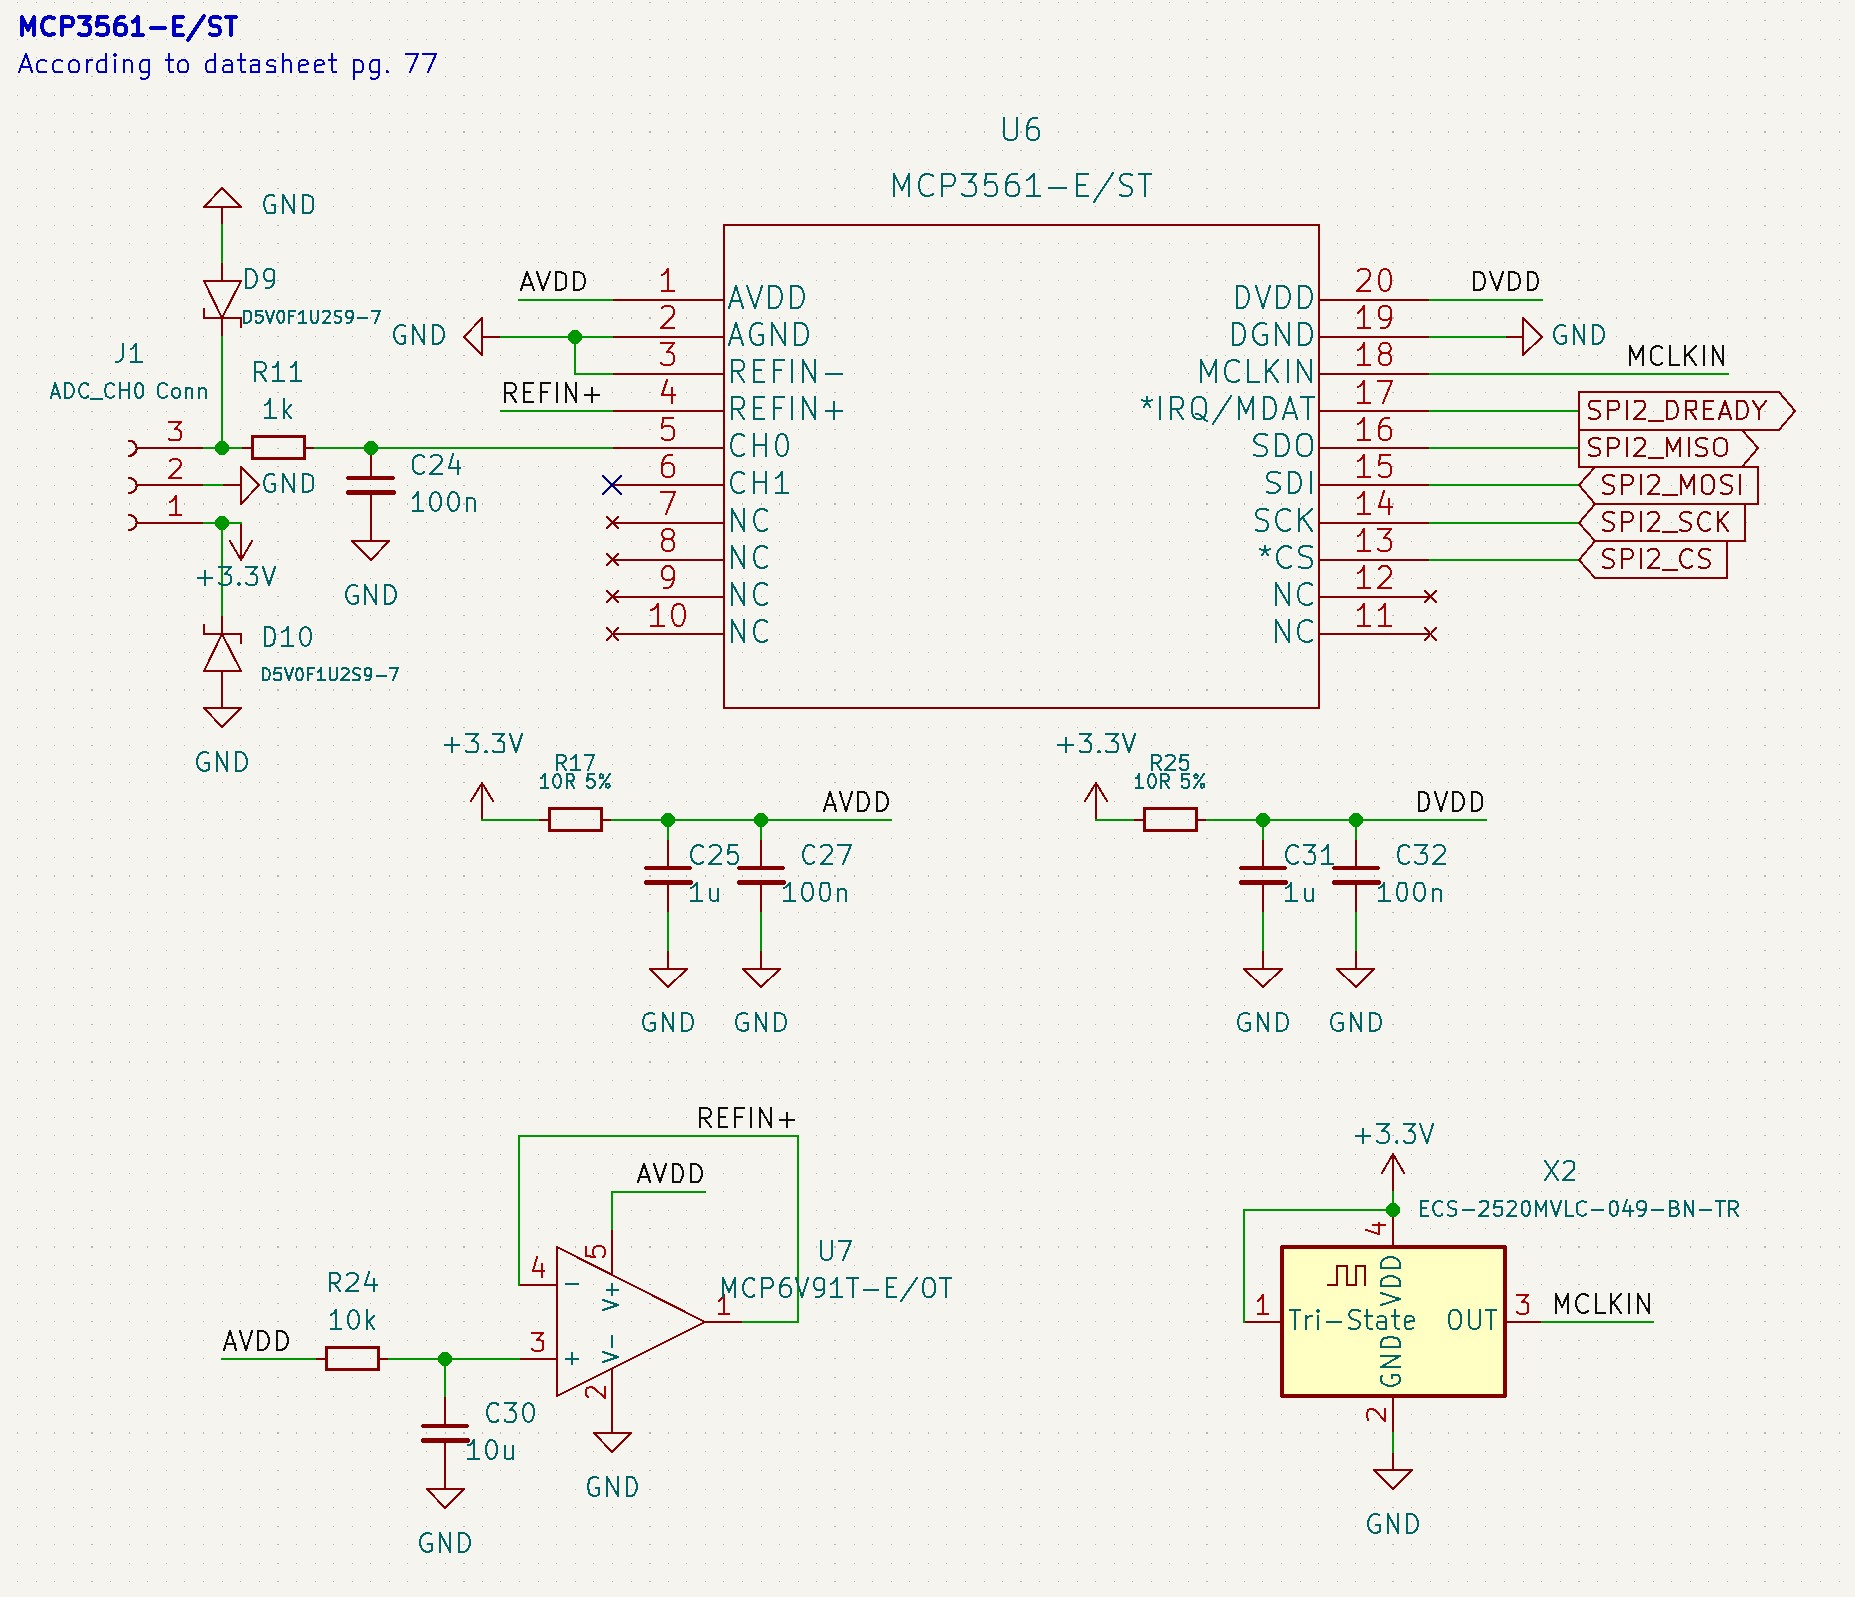
\includegraphics[width=1\linewidth]{pictures/mcp3561_connection.jpg}
\end{figure}
Na obrázku (\ref{fig:mcp3561_connection}) je schéma zapojení MCP3561 podle doporučeného zapojení výrobce.
\subsubsection{Napájení a napěťové reference}
Zapojení obsahuje oddělené filtrování analogového a digitálního napajecího vstupu. Je použit RC článek typu dolní propusti s parametry resistoru $R = 10 \ \Omega$ a kondenzátoru $C = 1100 \ nF$. Zlomová frekvence RC článku je $f_c \doteq 14.5 \ kHz$.
\par
Referenční napájení AD převodníku obsahuje operační zesilovač v zapojení napěťového sledovače, protože vstupní reference AD převodníku není impedančně oddělená. Operační zesilovač je MCP6V91T od firmy Microchip. Má nízkou teplotně závislou napětovou nesymetrii $U_{OS \ Drift} = \pm 17  \ \frac{nV}{^\circ C}$
a také nízkou napěťovou nesymetrii $U_{OS} = 9 \ \mu V$, nízký šum a je optimalizovaný pro použití v prostředí s vysokým elektromagnetickým prostředí.

\subsubsection{Externí oscilátor}
Místo interního oscilátoru AD převodníku je použit externí oscilátor ECS-2520MVLC od firmy ECS Inc. s frekvencí $f_{CLK} = 4.9152 \ MHz$. Externí oscilátor zaručí stabilní funkčnost AD převodníku, protože přesnost interního oscilátoru není výrobcem zaručena, rozdíly až $\pm 30  \ \%$, může se lišit čip od čipu, mohou způsobit vadnou komunikaci a další nepredikovatelné chování.
Podporované frekvence externího oscilátoru jsou v rozmezí $ 1 \ MHz \leq  f_{CLK} \leq 20 \ MHz $. Frekvence $f_{CLK} = 4.9152 \ MHz$ byla zvolena díky naměřených parametrů AD převodníku v katalogovém listu právě při použití této frekvence.
\par
Maximální možná přenosová rychlost pro tuto frekvenci oscilátoru je $f_s = 38400 \ Hz$.

\subsubsection{Přesnost a rušení}
Nejmenší možné snímané napětí ideálního $N = 24 - 1$ bit AD převodníku, protože rozah snímaného napětí je $\pm U_{ref}$ největší bit je rezervován pro znaménko. Při referečním napětí $U_{ref} = 3.3 \ V $ je $ 1 \ LSB = \frac{U_{ref}}{2^{N-1}} \doteq  393.390  \ nV$.
Efektivní počet bitů (ENOB) závisí na interní konfiguraci registrů MCP3561 a od toho se také odvíjí jaká přenosová rychlost bude mít nejlepší počet efektivních bitů. Přenosová rychlost udává počet vzorků odeslané po přenosové lince nadřazenému systému, signalizovaném výstupním digitálním pinem AD převodníku $\overline{IRQ}$.
Rovnice po výpočet přenosové rychlosti:
\begin{equation}
    f_s = DRCLK = \frac{DMCLK}{OSR} =\frac{f_{CLK}}{4 \times OSR \times Prescale}
\end{equation}
Rovnice je převzatá z katalogu AD převodníku. Kde $f_{CLK} = 4.9152 \ MHz$ je frekvence AD převodníku, DMCLK je vzorkovací frekvence AD převodníku, Prescale je hodnota pro decimaci taktovací frekvence AD převodníku s hodnotamy $PRESCALE = \{1, 2, 4, 8\}$.  OSR (Oversampling Ratio) je poměr vzorkovací frekvence ku přenosové rychlosti. Počet a hodnoty OSR jsou v omezeném množstvý a jsou napsané v katalogu AD převodníku. Podle katalogu závisí počet efektivních bitů a rušení na OSR.
Čím vyšší OSR, tím větší bude počet použitelných bitů a menší rušení. Pro dosáhnutí přenosové rychlosti $f_s = 5000 \ Hz$ byly vybrány hodnoty $Prescale = 1$, $OSR = 256$ a zesílení $Gain = 1 \times$. Vzorkovací frekvence AD převodníku je $DMCLK = \frac{f_{CLK}}{4 \times Prescale} = 1 \ 228 \ 800 \ Hz$ a výsledná přenosová rychlost je $f_s = DRCLK = 4800 \ Hz$. Výsledná přenosová rychlost vyhovuje požadavkům. Díky vybrání hodnoty OSR je výsledný $ENOB = 19.5 \ bit$ a RMS rušení $U_{noise \ RMS} = 8.94 \ \mu V$.
Výsledná přesnot AD převodníku se sníží na $ 1 \ LSB = \frac{U_{ref}}{2^{ENOB}} \doteq  4.4 \ \mu V$.
\par
K dalším parametrům AD převodníku MCP3561 patří
\begin{table}[H]
    \label{tab:mcp_adc_error}
    \caption{Charakteristika AD převodníku MCP3561. }
    % \centering
    \begin{itemize}
        \item $f_{CLK} = 4.9152 \ MHz$, $DU_{DD} = AU_{DD} = U_{REF} = 3.3 \ V$, $T = 25 ^\circ C$
    \end{itemize}
    \hspace*{-2cm}
    \begin{ctucolortab}
        \begin{tabular}{ccccccc}
            \toprule
            Charakteristika                           & Symbol                                   & Min                 & Typ               & $\textnormal{Max}$ & Jednotka                                          & \\ \midrule
            Impedance analogového vstupu              & $Z_{in}^{(\ref{enum:mcp_gain_one})}$     & -                   & 260               & -                  & $k \Omega$                                        & \\
            Rozlišení zavislé na OSR                  & $Rozlišení^{(\ref{enum:mcp_accuracy})}$  & 24                  & -                 & -                  & bit                                               & \\
            Napěťová nesymetrie                       & $U_{OS}$                                 & $\frac{-900}{GAIN}$ & -                 & $\frac{900}{GAIN}$ & $\mu V$                                           & \\
            Napěťová nesymetrie závislá na teplotě    & $U_{OS \ DRIFT}$                         & -                   & $\frac{70}{GAIN}$ & $\frac{300}{GAIN}$ & $\frac{nV}{^\circ C}$                             & \\
            Chyba zesílení                            & $G_E$                                    & -3                  & -                 & +3                 & \%                                                & \\
            Chyba zesílení závislé na teplotě         & $G_{E \ DRIFT}^{(\ref{enum:mcp_drift})}$ & -                   & 0.5               & 2                  & $\frac{ppm}{^\circ C}$                            & \\
            Integrální nelinearita                    & $INL^{(\ref{enum:mcp_gain_one})}$        & -7                  & -                 & +7                 & ppm $\textnormal{FSR}^{(\ref{enum:mcp_adc_fsr})}$ & \\
            Stejnosměrné potlačení souhlasného rušení & $DC \ CMRR$                              & -                   & -126              & -                  & dB                                                & \\
            Střídavé potlačení souhlasného rušení     & $AC \ CMRR$                              & -                   & 122               & -                  & dB                                                & \\
            Poměr signálu k šumu a zkreslení          & $SINAD$                                  & 105.8               & 106.7             & -                  & dB                                                & \\
            Poměr signálu k šumu                      & $SNR$                                    & 106.7               & 107.2             & -                  & dB                                                & \\
            Celkové harmonické zkreslení              & $THD$                                    & -                   & -116              & -111               & dB                                                & \\
            Dynamický rozsah bez parazitních složek   & $SFDR$                                   & 110                 & 120               & -                  & dB                                                & \\
            Přeslech vstupních kanálů                 & $CTALK$                                  & -                   & -130              & -                  & dB                                                & \\
            \bottomrule
        \end{tabular}
    \end{ctucolortab}
    \begin{enumerate}
        \item Gain = 1 \label{enum:mcp_gain_one}
        \item OSR $\geq$ 256 \label{enum:mcp_accuracy}
        \item Gain = 1,2,4 \label{enum:mcp_drift}
        \item Full-Scale-Range(FSR) = $2 \times U_{REF}/GAIN$ \label{enum:mcp_adc_fsr}
    \end{enumerate}
\end{table}


\section{Datové úložiště}
Přidané datové úložitě slouží jako úložiště dat z AD převodníku MCP3561. MCU příjmá data o velikosti $N = 24 bit$ při přenosové rychlosti $f_s \approx 5000 \ Hz$ po dobu $T = 30 \ s$. Velikost úložiště je potřeba alespoň
\begin{equation*}
    M = N \times f_s \times T = 3 \ 600 \ 000 \ bit
\end{equation*}
Neboli $\frac{M}{8} = 450 \ kB$.
\par
Interní úložiště MCU STM32F407ZG6 typu FLASH je 1 MB, ale toto úložistě slouží jako úložiště programu a také sdílí s periferiemy MCU. Dostupné interního úložistě MCU je menší než potřebné.
\par
Jako přidané datové úložiště je vybrána NOR FLASH paměť MX25R3235FM2IH0 od firmy Macronix o velikosti 32 MBit. Komunikace probíhá přes komunikační protokol SPI. NOR FLASH je typ energeticky nezávislou paměť, po odpojení napájení stále drží zapsaný obsah.
\begin{figure}[H]
    \label{fig:flash_memory}
    \caption{Schéma zapojení paměti flash Macronix MX25R3235FM2IH0}
    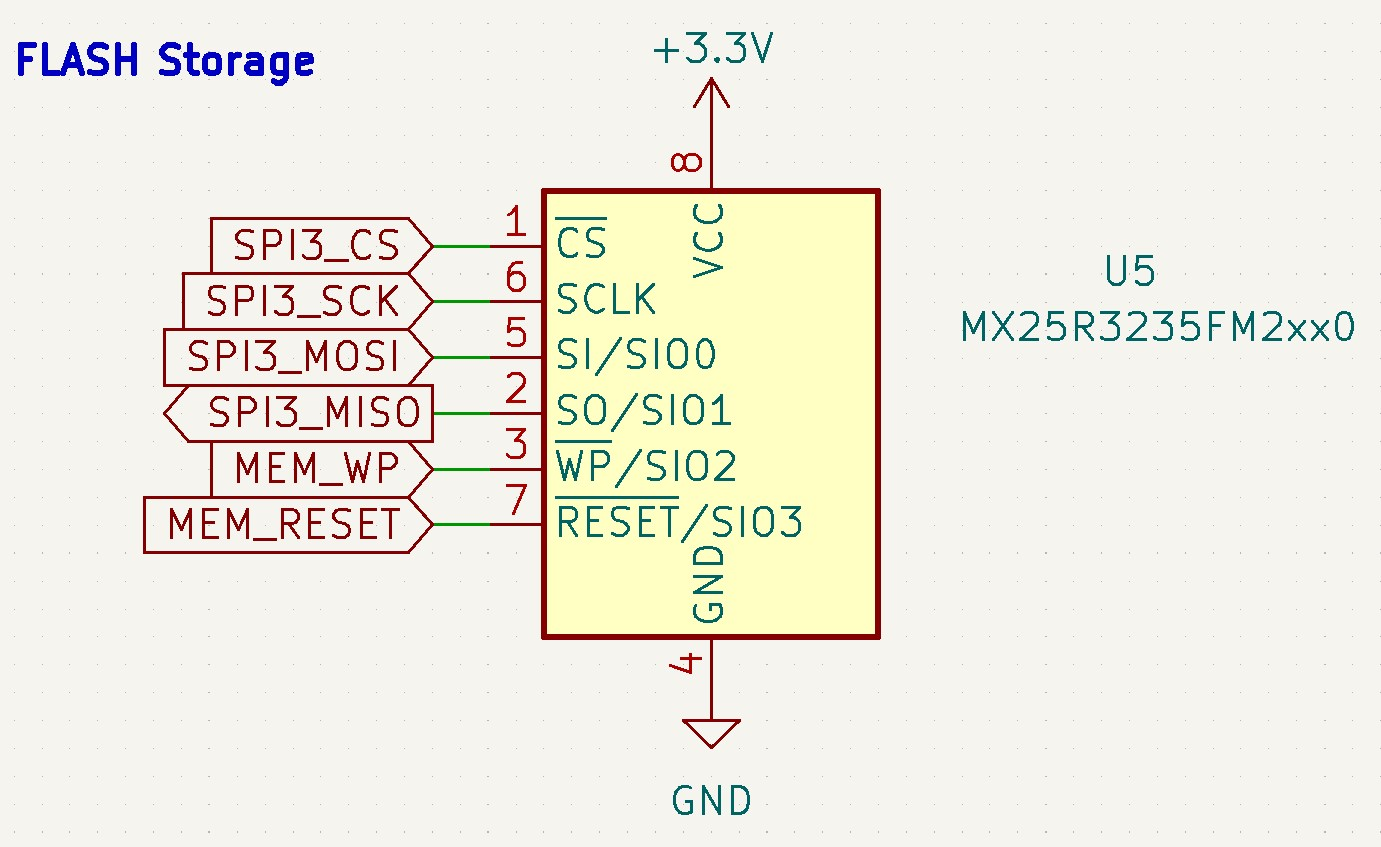
\includegraphics[width=1\textwidth]{pictures/flash_memory.jpg}
\end{figure}
Paměť je rozdělena do 64 kB bloků, které jsou poté rozděleny do bloků po 32 kB, ty do 4 kB sektorů. Do paměti je nejmenší možný zápis po 256 B stránkách. Přenosová perioda příchozích 24 bit dat z AD převodníku je $t_s = 208 \ \mu s$ a doba pro zápis celé stránky je $t_{PP} = 850 \ \mu s$. 256 B příchozích z AD převodníku je za $t_p = 256 \times \frac{t_s}{3} \doteq 17.7 \ ms$.
Použitá paměť nám umožní bezpečně uložit data s dostatečnou prodlevou před příchozí další 256 B z AD převodníku.
\section{Nouzové zastavení}
V situaci, kdy pacient se během terapie cítí v ohrožení nebo kdy se děje s přístrojem něco mimo běžného stavu, je přístroj vybaven obvodem pro připojení nouzového tlačítka.
\begin{figure}[H]
    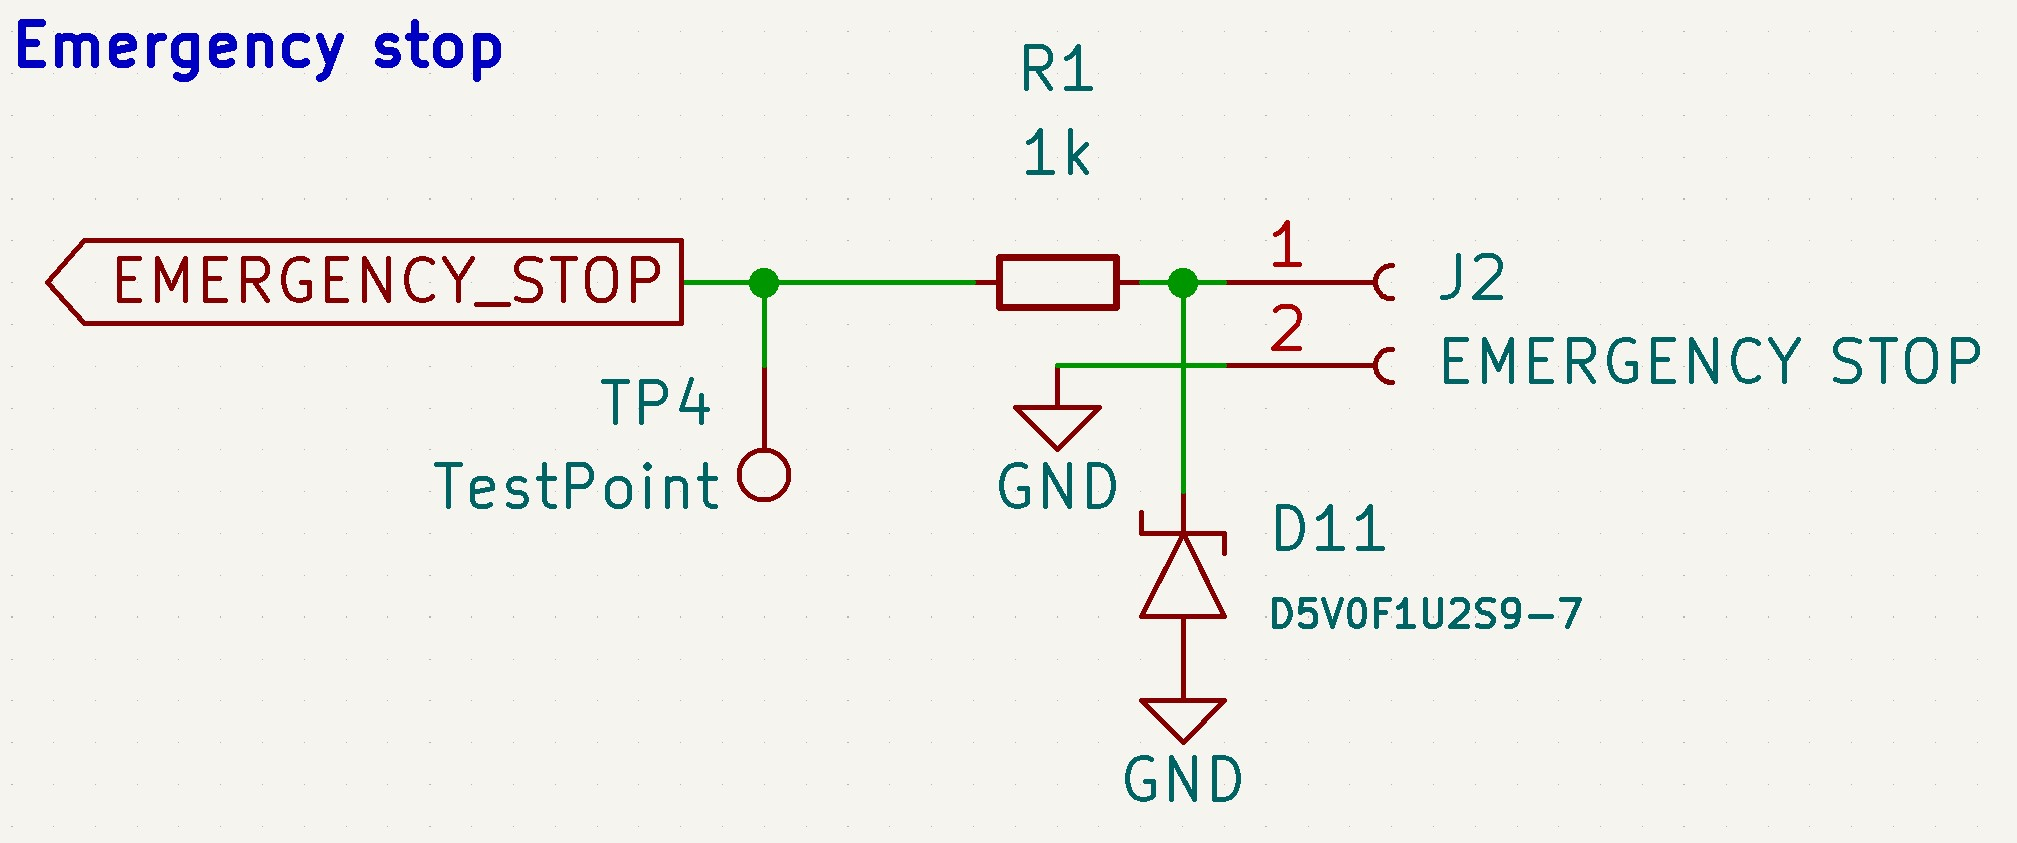
\includegraphics[width=0.9\linewidth]{pictures/e_stop.jpg}
    \caption{Schéma zapojení nouzového tlačítka}
    \label{fig:e_stop}
\end{figure}
Nouzové tlačíko je připojeno ke vstupními pinu MCU, které má k dispozici externí přerušení. Pin MCU musí mít pull up rezistor a přerušení nastavené na detekci spádové hrany. Toto nastavení zajístí
detekci odpojeného nouzového tlačítka, přístroj se programově nastaví do stavu nouze a tím uživateli přístroje zabrání spuštění terapie bez zabezpečení proti selhání.
\section{Napájení}
Vstupní napájení je použito pro napájení celého přistroje. Vstupní napětí je $U_{in} = 5V DC$, které poskytuje napájení pro všechny součástky na přístroji. Vstupní napětí je poté pomocí regulátoru napětí s nízkým úbytkem usměrněno na $3.3 V$ pro napájení MCU, sensorů a ostatních komponentů.

\begin{figure}[H]
    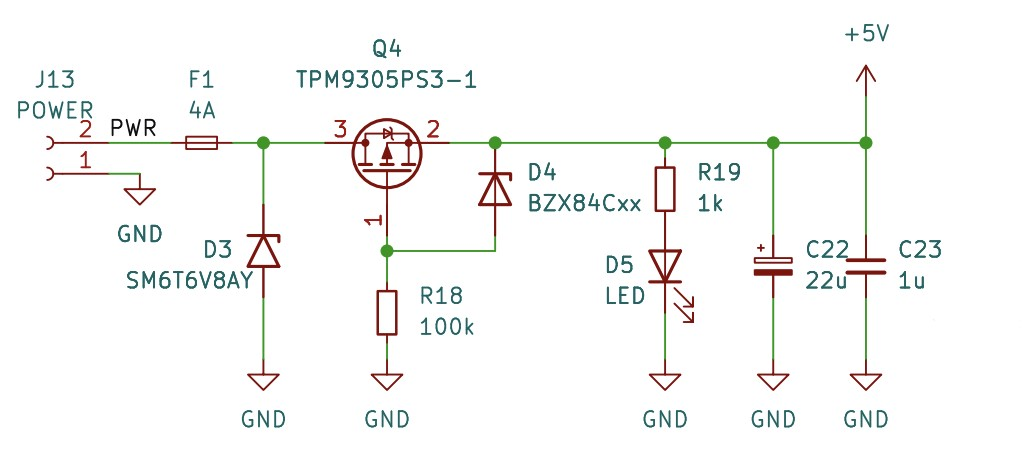
\includegraphics[width=0.9\linewidth]{pictures/power.jpg}
    \caption{Schéma zapojení vstupního napájení}
    \label{fig:power_input}
\end{figure}

Celkový proudový odběr přístroje je
\begin{table}[H]
    \label{tab:sum_of_current}
    \caption{Celkový proudový odběr přístroje}
    % \hspace*{-1.2cm}
    \centering
    \begin{ctucolortab}
        \begin{tabular}{cccccc}
            \toprule
            Komponenta              & Název                 & Symbol & Hodnota & Jednotka \\ \midrule
            Diferenční sensor tlaku & Amphenol ELVH-L02D    &        & 35      &          \\
            Sensory tlaku           & NXP MP3V5050GC6U      &        & 20      &          \\
            Uzavírací ventily       & Conjoin CJAV08-2B05A1 &        & 401     &          \\
            Regulační ventily       & JQF4-6A/DC6V          & I      & 214     & mA       \\
            Modul měření BP         & PAR NIBP 2020 UP      &        & 1000    &          \\
            MCU                     & ST M STM32F407ZG6     &        & 109     &          \\
            AD převodník            & Microchip MCP3561     &        & 2.2     &          \\
            FLASH Paměť             & Macronix MX25R3235F   &        & 2       &          \\
            \bottomrule
            $\Sigma$                &                       &        & 1.7922  & A        \\
            \bottomrule
        \end{tabular}
    \end{ctucolortab}
\end{table}

Přístroj je opatřen $4 \ A$ pojistkou a ochranou proti opačné polaritě.
Ochrana proti opačné polaritě zajistí při špatném zapojení, aby proud neprotékal přístrojem, ale musí se zajistit, aby ztrátový výkon
\begin{align*}
    W = I^2 R
\end{align*}

byl co nejmešní při správném zapojení. Proto je použit PMOS tranzistor jako ochrana obvodu, který . Gate tranzistoru je připojena k zemi a mezi Drain a Source protéká proud při správném zapojení napájecího zdroje. Protože $ U_G = 0 [V]$ a $U_S = U_{in}$, tak
\begin{align*}
    U_{GS} = U_G - U_S
\end{align*}
$U_{GS} = -U_{in} $, proto je potřeba, aby
\begin{align*}
    U_{GS(ON)} > -U_{in}
\end{align*}
Při opačném zapojení napájení $U_S = -U_{in}$ a $ U_G = 0 V$, tak  $U_{GS} = U_{in}$ tranzistor je vypnut a přes obvod neprotéká proud.
V návrhu je použit tranzistor TPM9305PS3, který má  $U_{GS(ON)} = -2.5V $,  $I_D = -4.1A$ a $R_{DS(ON)} = 52m \Omega$ při $U_{GS} = -4.5V$.
Ztrátový výkon bude
\begin{align*}
    W_{loss} = I^2 R \approx (3)^2 (0.053) =  159 mW
\end{align*}

Na obrázku (\ref{fig:power_input}) je ještě připojena mezi $U_G$ a $U_S$ zenerova dioda, která zamezí maximální napětí, pro ochranu tranzistoru. Pokud napájecí zdroj bude mít větší napětí něž maximální povolené napětí na $U_{GS}$, zenerova dioda upne $U_{GS}$ na její maximální napětí.
\par
Pro maximální zamezení rušivých jevů a braní ohledu na EMC jsou připojeny paralelně dva blokovací kondenzátory.

\begin{figure}[H]
    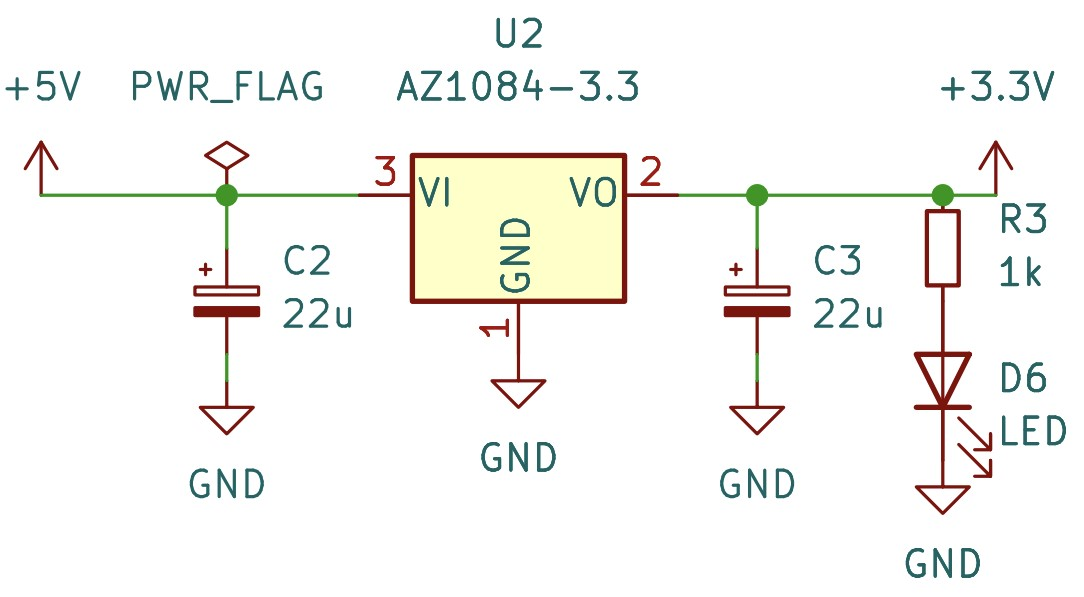
\includegraphics[width=0.9\linewidth]{pictures/ldo_3v3.jpg}
    \caption{Schéma zapojení regulátoru napětí z 5V na 3.3V}
    \label{fig:stepdown}
\end{figure}
Na obrázku (\ref{fig:stepdown}) je schéma zapojení lineárního regulátoru napětí s nízkým úbytkem AZ1083-3.3. Vstupní napětí je v rozmezí $1.5V \leq U_{in} \leq 12V $. Výstup regulátoru je fixní na $U_{out} = 3.3V$ a maximální výstupní proud je $I_{out(MAX)} = 5A$. Zapojení regulátoru je podle doporučeného zapojení v katalogového listu.


